\documentclass[12pt,a4paper]{article} 

% Please add the following required packages to your document preamble:
%\usepackage[table,xcdraw]{xcolor}
\usepackage{xcolor}
% If you use beamer only pass "xcolor=table" option, i.e. \documentclass[xcolor=table]{beamer}
\usepackage[normalem]{ulem}
\useunder{\uline}{\ul}{}
\usepackage{graphicx}
\usepackage[utf8]{inputenc}
\usepackage[T1]{fontenc}
%%\usepackage{style}%%

\usepackage[a4paper,pdftex,vmargin=3.5cm]{geometry}		
%\usepackage[margin=20mm]{geometry}	
								% A4paper marginshttps://preview.overleaf.com/public/hyschynkprmv/images/ca4ec9bd02dd412a4bb2fe023daaa85ee9a14380.jpeg
\setlength{\oddsidemargin}{5mm}												% Remove 'twosided' indentation
\setlength{\evensidemargin}{5mm}
\usepackage{booktabs}
\usepackage[protrusion=true,expansion=true]{microtype}	
\usepackage{amsthm}
\usepackage[T1]{fontenc}

\usepackage{lmodern}
\usepackage{hyperref}
%\usepackage[latin1]{inputenc}
\usepackage[]{units}
\usepackage{pdfpages}
% Swift syntax highlight definition for listings
\usepackage{listings}
\lstdefinelanguage{swift}
{
  morekeywords={
    open,catch,@escaping,nil,throws,func,if,then,else,for,in,while,do,switch,case,default,where,break,continue,fallthrough,return,
    typealias,struct,class,enum,protocol,var,func,let,get,set,willSet,didSet,inout,init,deinit,extension,
    subscript,prefix,operator,infix,postfix,precedence,associativity,left,right,none,convenience,dynamic,
    final,lazy,mutating,nonmutating,optional,override,required,static,unowned,safe,weak,internal,
    private,public,is,as,self,unsafe,dynamicType,true,false,nil,Type,Protocol,
  },
  morecomment=[l]{//}, % l is for line comment
  morecomment=[s]{/*}{*/}, % s is for start and end delimiter
  morestring=[b]", % defines that strings are enclosed in double quotes
  breaklines=true,
  escapeinside={\%*}{*)},
  numbers=left,
  captionpos=b,
  breakatwhitespace=true,
  basicstyle=\linespread{1.0}\ttfamily\footnotesize, % https://tex.stackexchange.com/a/102728/129441
}

\definecolor{keyword}{HTML}{BA2CA3}
\definecolor{string}{HTML}{D12F1B}
\definecolor{comment}{HTML}{008400}

\lstset{
  language=swift,
  basicstyle=\ttfamily\small,
  showstringspaces=false, % lets spaces in strings appear as real spaces
  columns=fixed,
  keepspaces=true,
  keywordstyle=\color{keyword},
  stringstyle=\color{string},
  commentstyle=\color{comment},
}
%importera paket. L�gg till paket i filen style
%\usepackage{style}

% ------------------------------------------------------------------------------
% Definitions (do not change this)
% ------------------------------------------------------------------------------
\newcommand{\HRule}[1]{\rule{\linewidth}{#1}} 	% Horizontal rule
\newcommand{\imageSize}{256x256 }

\newcommand{\floor}[1]{\left\lfloor #1 \right\rfloor}
\newcommand{\ceil}[1]{\left\lceil #1 \right\rceil}


\makeatletter							% Title
\def\printtitle{%						
    {\centering \@title\par}}
\makeatother									

\makeatletter							% Author
\def\printauthor{%					
    {\centering \large \@author}}				
\makeatother							

% ------------------------------------------------------------------------------
% #################### Metadata (Change this) ####################
% ------------------------------------------------------------------------------
\title{	\normalsize \textsc{Lund University\\
Lunds Tekniska Högskola\\
Centre for Mathematical Sciences
} 	% Subtitle of the document
		 	\\[2.0cm]													% 2cm spacing
			%\HRule{0.5pt} \\										% Upper rule
			\LARGE \textbf{\uppercase{ Object Detection In Augmented Reality\\Project report\\~\\ }}	% Title
			\HRule{2pt} \\ [0.5cm]								% Lower rule + 0.5cm spacing
			\normalsize Hand-in date:	\today								% Todays date
		}

\author{
		Jan Svensson, \texttt{elt12jsv@student.lu.se} \\
        Jonatan Atles, \texttt{elt13jat@student.lu.se} \\
}
\pagenumbering{gobble}
%https://www.overleaf.com/8187414vnsqvdmvvcyt for sharing rwx :)
\begin{document}

\printtitle									% Print the title data as defined above
 	\vfill
\printauthor								% Print the author data as defined above
%
\newpage %------------------------------------------------------------------------------
% ###### Begin document ######
% ------------------------------------------------------------------------------

 
% Underubrikerna ska vara:
% Abstract
% Table of contents
%  Förord
% Inledning
% Metodik
% Diskussion/slutsats
% hämta externa filer
%\newpage
\pagenumbering{roman}

\begin{center}
\section*{Abstract}
Augmented reality is a field which is getting increased funding every year, as more businesses are realizing the potential of rendering virtual objects in the real world. As the equipment gets more commercialized, the costs will get lowered while performance also goes up. As of now, augmented reality only makes use of plane detection and marker detection to find and locate objects. We want to incorporate machine learning using deep neural networks to be able to find objects in an augmented reality scene. 

In this report we go through the process of developing an an iOS application, which incorporates use of object detection, object recognition and augmented reality. Our goal is to identify if the combination of these field is both feasible and desirable with modern tools available.The application is supposed to work as an alternative to conventional assembly manuals for furniture. 

The final product makes use of \textit{ARKit} developed by \textit{Apple} to render the augmented reality scene, and \textit{Apple's} \textit{Turi Create} to train a neural network for object detection and classifier. 

We then evaluate the performance by having users of various backgrounds perform user tests. We conclude that modern technology makes our idea possible and the user tests shows that the concept has great potential and is desirable.
\end{center}



\newpage
\section{Preface}

\newpage
\tableofcontents
\newpage
\pagenumbering{arabic}
\section{Introduction}
To first get an understanding of why this project was done, it is important for the reader to learn, not only the background of the fields studied, but also about the prospects of the technologies involved.
 At \hyperref[subsecBackground]{3.1} we go through the current and the potential use of these technologies; also what prospects the consumers and the industry has. Later on, at  \hyperref[subsecPrevStud]{3.2} we go through some of the previous research that has been done in the fields that are studied in the report. This section is then rounded of at \hyperref[subsecGoal]{3.3} with us telling you what we hoped to achieve with this project and a brief run-down of how.

\subsection{Background}
\label{subsecBackground}
Why is AR and Object recognition interesting, for the consumers and Jayway

The idea of Augmented Reality is to render virtual object in the real world. This usually requires hardware in the form of a camera and display, a processing unit and software. Common AR devices today are the HoloLens \cite{microsoft}, Google's Glass \cite{googleGlasses} and a vast amount of mobile devices, such as Apple's iPhone X \cite{appleAR}. 

The general interest for AR has undeniably grown in recent years, with mobile games and applications such as Niantic's Pokémon Go \cite{pokemonGO} and IKEA's IKEA Place \cite{IKEAPlace} the AR industry has peaked a general interest and sources speculate it could be a \$90 million dollar industry by 2022 \cite{digi-capital}.
 But Augmented Reality has not only reached the casual users; the technology has also peaked an interest in several industries. One such project is Fieldbit's Fieldbit Hero \cite{fieldbit}, a platform enabling technicians to get instant AR annotations to their AR devices from an engineer, allowing the technician to get visual instructions while simultaneously  being able to work hands-free. 
 
[SKRIVA MER OM OBJECT DETECTION OCH OBJECT RECOGNITION]

\subsection{Previous studies}
\label{subsecPrevStud}
D. Chatzopoulos et al.(2017) describes the basics of Mobile Augmented Reality, its advancements and it's flaws. They estimate that MAR is the most promising field of mobile applications and that it will have a massive impact on how we interact with the real world. However, they also go through some of the current hiccoughs with the technology, such as bandwith limitation and the computing power required. 
\cite{MARS}

S.Gould et al.(2009) writes about a hierarchical model for joint object detection and image segmentation, where they basically tried to segment all objects in an image and classifies every pixel. 
\cite{NIPS2009_3766}


Y LeCun and M.A. Ranzato goes in-depth on the history and progress of deep learning, from the first machine learning model, the Perceptron, to future challenges with deep learning. They write about the use cases for machine learning and how models generally work. They also classify different kinds of models into separate categories. Also written about is areas such as what makes a good feature and how convolutional neural networks are constructed.
\cite{deepLearningTutorial}


\subsection{The goal of this project}
\label{subsecGoal}
When working with Augmented Reality it is obviously interesting to know where planes are and how the camera moves in the scene to be able to render virtual object. But usually there is more than one single plane in ones environment. Usually there are other objects in the scene that affects how the virtual objects should be rendered. Sometimes maybe the virtual objects could interact with the real objects to make a more realistic scene. Because of this it can be very interesting to know what those objects actually are.

For example, if you are going to place a virtual furniture in your home it would be good to detect other furnitures in the area so that the virtual object can collide with the real object. This way, they will not intertwine with each other.

% Our master thesis
Or maybe one would like to give virtual instructions to a user for assembling or constructing a certain product or to do maintenance. It is then important to figure out what 3D objects there are in the scene to be able to render instructions on the right places.

Augmented Reality technology has come a long way, but there are still things missing for making it a genuine experience. In ARKit, for instance, if a virtual object is rendered on top of a plane and a real object come in between the virtual object will still be rendered first. This makes it painfully obvious that the virtual object is just a 2D drawing on the screen.

\begin{figure}[hbtp]
\begin{center}
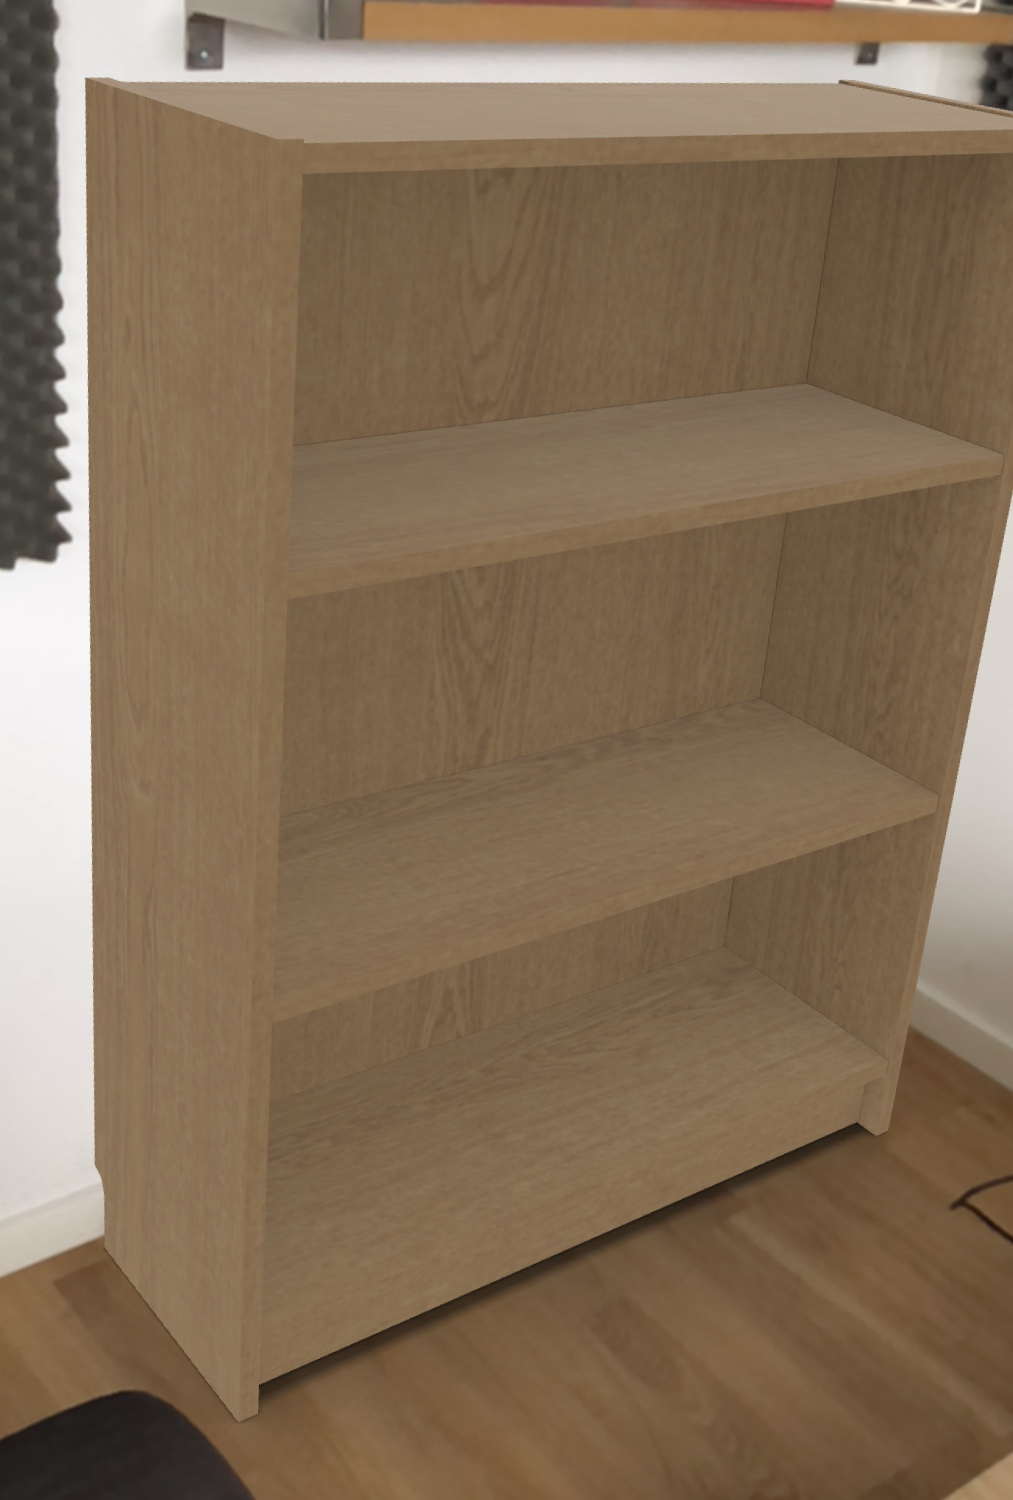
\includegraphics[width = 0.25\textwidth]{./Images/overlapping2.jpg} 
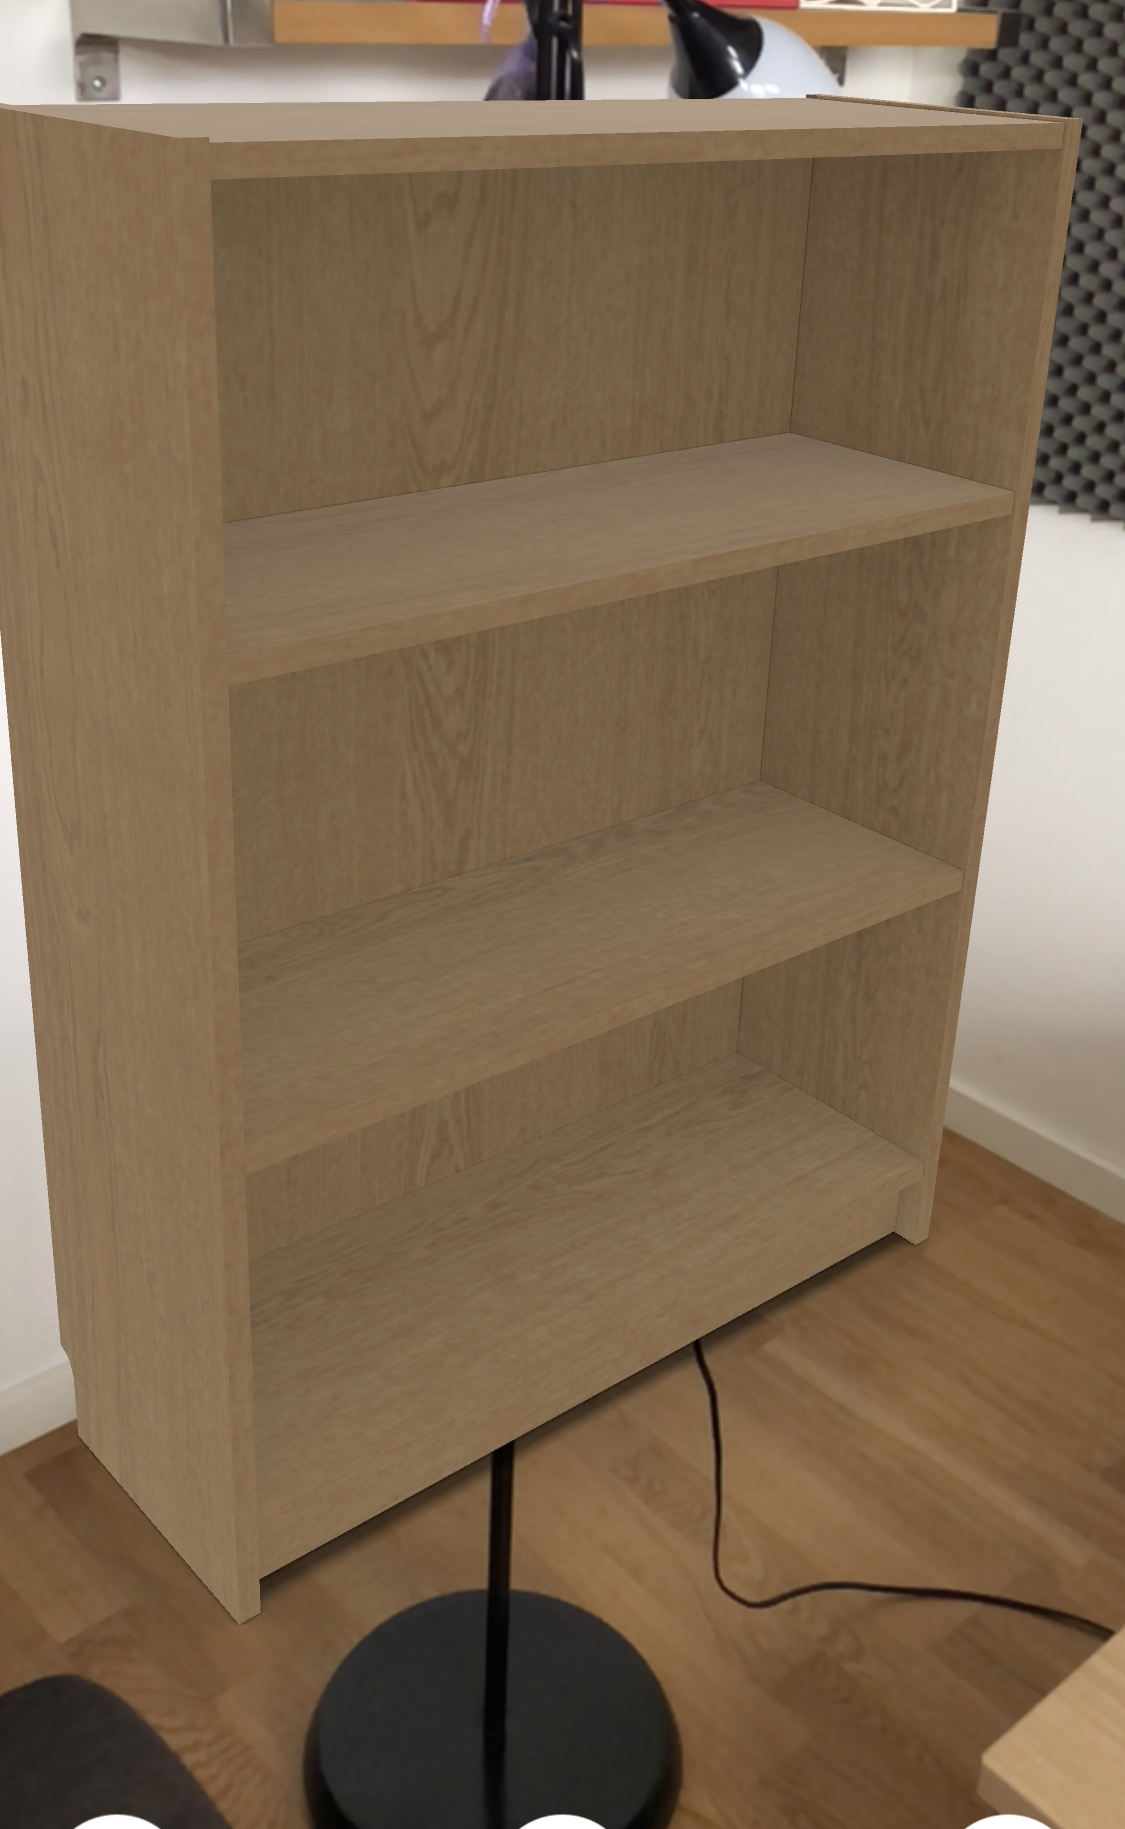
\includegraphics[width = 0.25\textwidth]{./Images/overlapping1.jpg} 
\caption{Book shelf rendered in a corner. To the left no objects in front so it looks realistic.On the right, the book shelf has a lamp in front of it.}
\end{center}
\end{figure}

Our goal is to try to combine Augmented Reality with Object detection and Object recognition to see if there is a possibility to create something valuable out of this. This report will investigate both the performance possibilities and the creative possibilities as well as research the current tools and try to push them to their limits.


\newpage

\chapter{Project Methodology}

When working in a project it is generally a good idea to work according to a predetermined project methodology model. This tends to make the work more effective and produce better quality. That is, more is produced during the same amount of time, the final product is more thought out, better teamwork etc.

Simply, if you have a plan at the start it is easier to stick to that plan and stay on the same path as intended, rather than shifting to another one. That is not to say that the plan cannot change, but if it does it does so controllably.

A historically good model has been the waterfall model. However, in the software industry this has changed lately with the agile methodology being more popular and it has proven to be very effective.

\section{Agile}
Basically, the agile model says that rather than planning a workload for 6 months forward or so it is better to work in short iterations. These iterations should be between 1 - 4 weeks depending on the team.
Instead of trying to estimate the time it will take to complete an entire project, the team is given a finite time frame and tries to complete as much as possible during that time. During this time, the team works very closely to the customer and project owner to make sure that they will get what they want and ask for.
For selecting items to work with for every sprint the team keeps a backlog of items it wishes to complete during the project. Every sprint, these items or stories are picked out and included into the sprint and estimated in size. The stories themselves should be collected from customers, project owner, users and people connected to the product. This way, the team knows what the purpose of developing a certain thing is. If there is any doubt about a specific feature it should be easier to ask than to assume.

This is of course a simplified version of how the agile method works.
'Extreme Programming Pocket Guide' is a good book for anyone who wants to read more about agile methodology.\cite{extremeProgramming}

\section{How we used the agile methodology}
\textbf{Sprints} \\
For our planned work we have decided to work in two week period sprints. At each start of a sprint we pick out stories to focus on for the coming two weeks and try to estimate how long each of them will take.
On weekdays we start with a quick discussion about yesterdays work and what we are planning to do today. This is for everyone to be up to speed about the other person's work.
At the end of the sprint everything is reviewed and analyzed so to do even better the next sprint by correcting possible faults.\\

\textbf{Story board} \\
For organizing our sprints we used a story board which contained an area for our backlog items and four rows for our stories during a sprint. The stories were broken into tasks which were placed on either one of the columns (Started, In Progress, Waiting, Completed).
Each story was estimated with a size which was a number in the fibonacci sequence. Each story was also divided into 5 parts (Started, Halfway done, Completed, Reviewed, Verified). These two numbers were multiplied and summed up with all the other stories to get how many points the sprints had. As we worked these points were subtracted and ultimately hit zero when we were done with everything. We plotted the progress on a chart as well for graphic. This is called a burndown.

\begin{figure}[hbtp]
\begin{center}
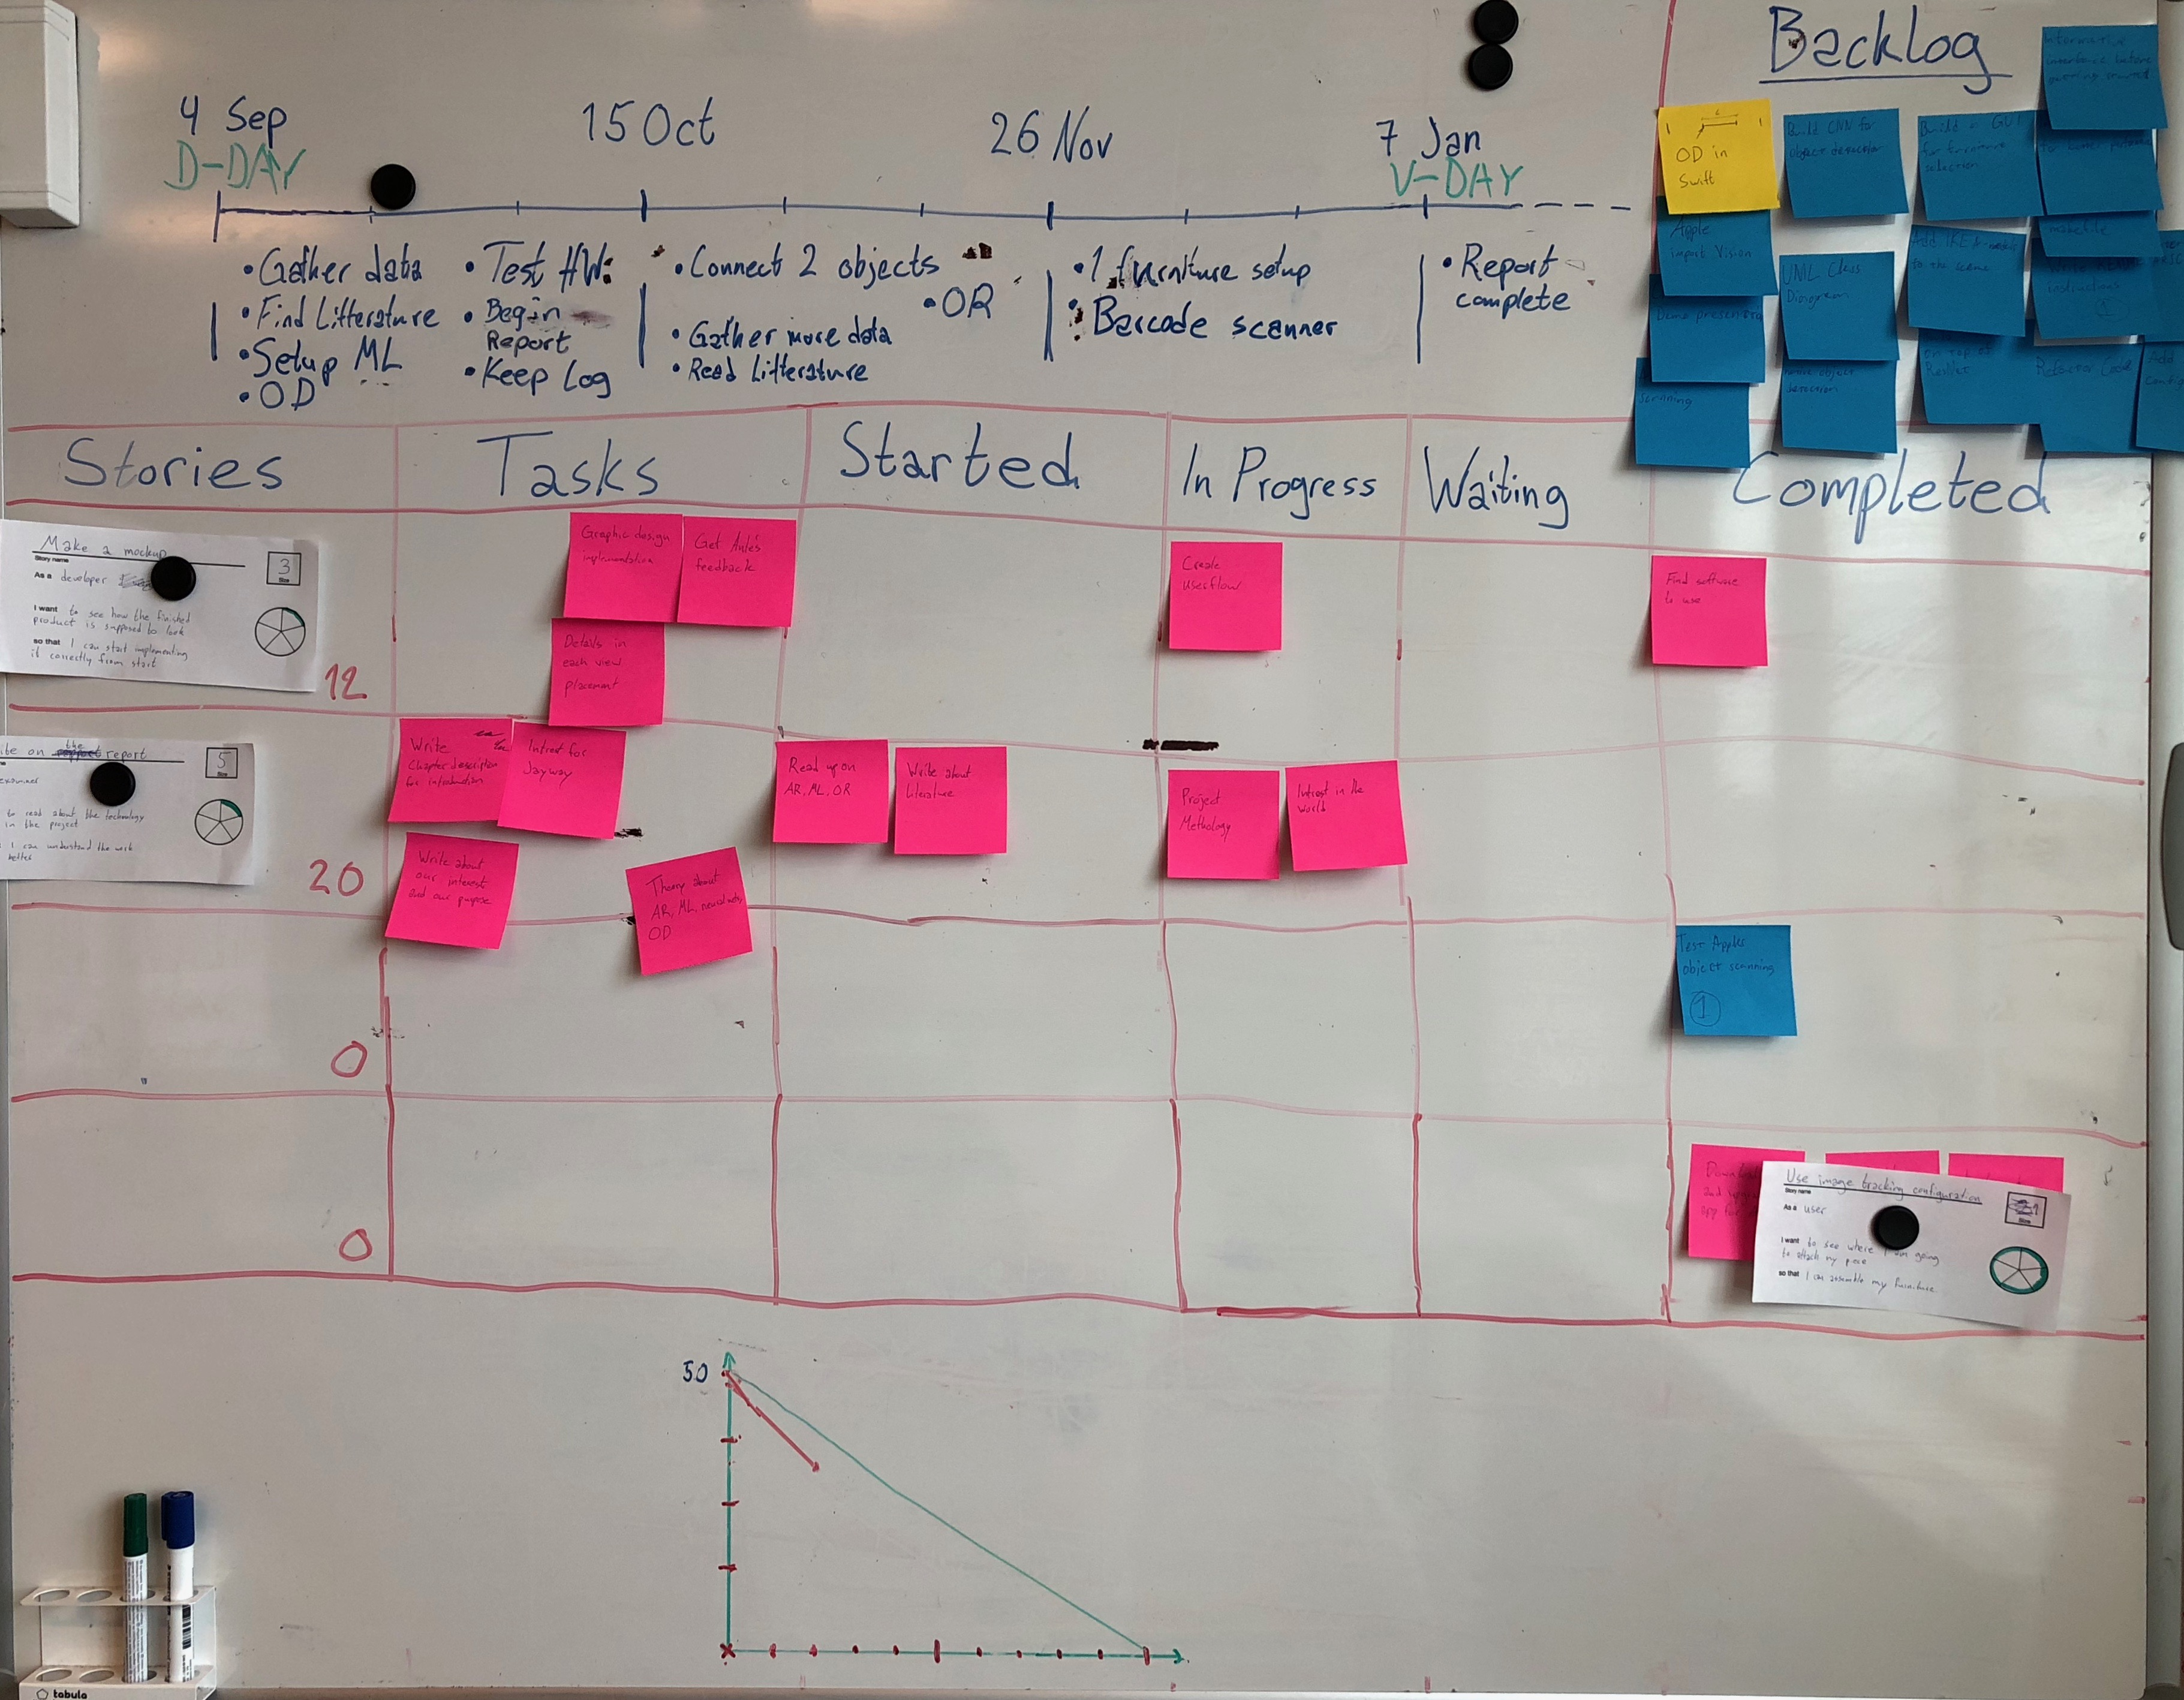
\includegraphics[width = 0.5\textwidth]{./Images/story_board.jpg} 
\caption{Story board used during the project}
\end{center}
\end{figure}


\textbf{Close relationship with project owner} \\
We worked very close to the project owner by sitting on desks right across him. Whenever we had a questing we could simply raise our head and ask it.

\newpage
\chapter{Augmented Reality}

Introtext to chapter
\section{How does Augmented Reality work?}
There are different types of augmented reality. Some of those are marker-based, location-based, superimposition-based and projection-based. \\

\textbf{Marker-based} AR is when markers, in the form of images have to be placed in the real world and detected by the application. Virtual object are rendered on top of these markers. An example would be a picture in a magazine which, when pointing a camera at it, the application renders an 3D object on top. An example is shown in figure \ref{fig:marker-based-ar} \\

\begin{figure}[hbtp]
\begin{center}
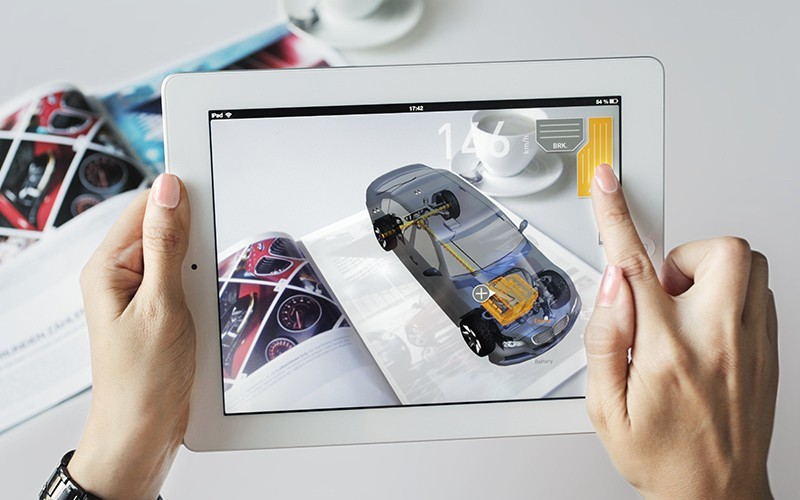
\includegraphics[width = 0.75\textwidth]{./Images/markerbasedar.jpg} 
\caption{A virtual object in the form of a car being rendered on top of a marker in a magazine.}
\label{fig:marker-based-ar}
\end{center}
\end{figure}

\textbf{Location-based} AR is when the content on the users screen differs depending on the location of the user. This type is highly dependent on the GPS signal.
An example of where this could be useful is in a museum where different information could be given to the user depending on which room he is in.\\

\textbf{Superimposition-based} AR uses object recognition in order to enhance that object with some sort of visual information. It replaces the real object with an enhanced virtual one. It could be used in retail to display different patterns on a piece of clothing.\\

\textbf{Projection-based} AR is when virtual object can be placed in a room to make it appear as if they were there. A popular example of this would be the IKEA Place app that was mentioned in the introduction. An example is shown in figure \ref{fig:projection-based-ar} \\

\begin{figure}[hbtp]
\begin{center}
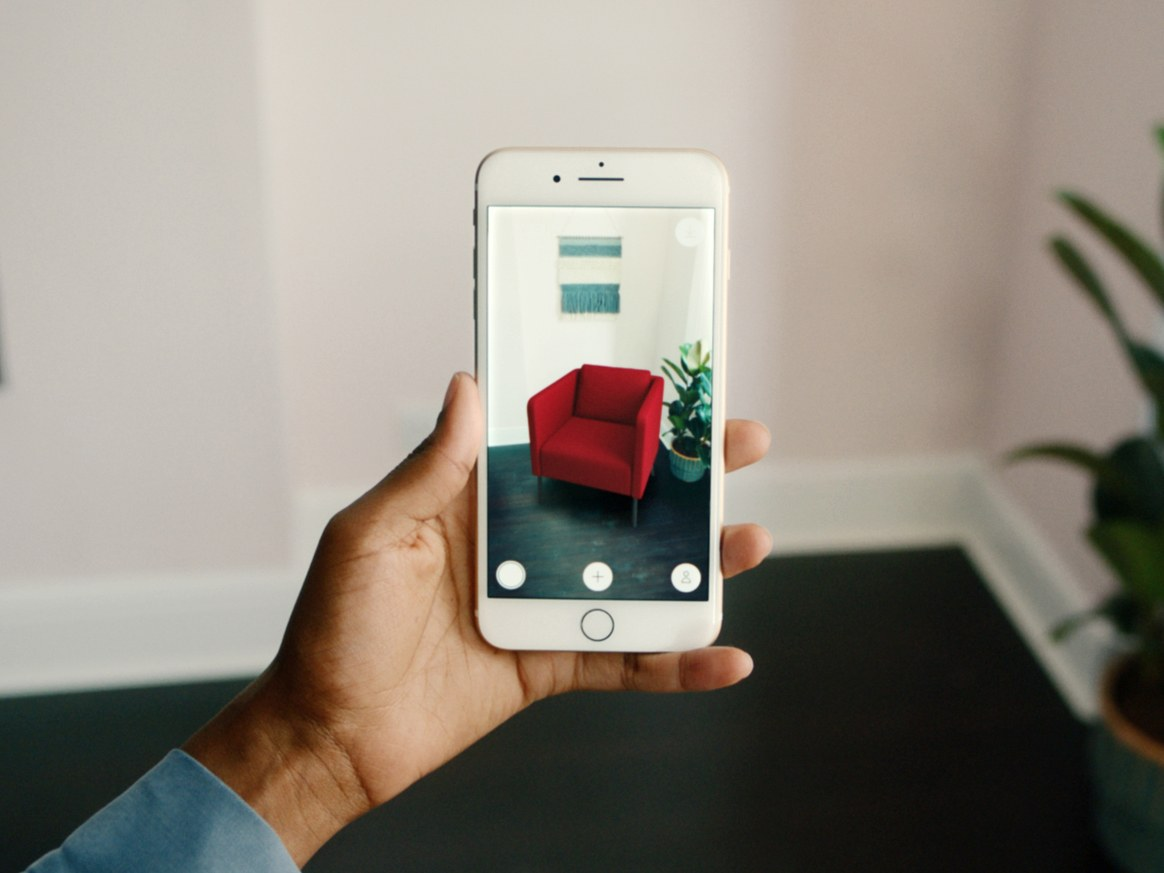
\includegraphics[width = 0.75\textwidth]{./Images/ikeaplace.jpg} 
\caption{A virtual sofa chair being added to a room within the IKEA Place app.}
\label{fig:projection-based-ar}
\end{center}
\end{figure}

In this paper we will mainly be using projection based AR with a form of recognition. The projections will be in the form of way-pointers used as instructions for the user to perform the next step in putting together a furniture piece. These instructions can visualize how the pieces will look like after the step is completed, and to show arrow pointers between the pieces that are supposed to be put together.

\subsection{History of AR}
The idea of augmented reality has existed a long time, the phrase has only been used for about 30 years but it is not until recently that the technology has become mainstream.
This is mainly due to it becoming good enough to be used by the average person at home. Today we can just download an app on our smart phones to enjoy the technology. Below follows a brief history of how augmented reality has progressed throughout the years.\\

\textbf{1968}
The Sword of Damocles - The first mounted headset.
This device was mounted on the head and could display a cube wireframe floating in the air. It was invented by Ivan Sutherland.\\

\textbf{1975}
Myron Krueger - Videoplace. Using cameras to interact with a digital world with shadows.
This application could be used to draw things or play simple video games with the shadow of your hand.
\cite{videoplace}\\

\textbf{1990}
The first time the term "Augmented Reality" was used by the Boeing researcher Tom Caudell.\\

\textbf{2009}
AR comes to the web in the form of an open source toolkit called ARToolKit.\\

\textbf{2017}
Apple launches AR Kit and Google launches AR Core.\\

\subsection{S.L.A.M.}
S.L.A.M (Simultaneous Localization and Mapping) is a way for a machine to get to know the environment that it is in. It registers features and maps them to its surroundings. S.L.A.M is about having the map of the environment and knowing where the robot is in that map.
The problem with this is that a map is needed for knowing where you are, and you have to know where you are to be able to create a map. That is why S.L.A.M is doing this at the same time, hence 'Simultaneous'. The system is used in autonomous robots, but also valuable in Augmented Reality. \cite{slam}
In figure \ref{fig:slam} a robot is driving around in a room collecting data. The robots camera can be seen in the lower left corner.

iPhone X does this by tracking multiple reference points in space and from them building a 3D model of the surroundings using a form of S.L.A.M technique.
This is accomplished by keeping a map of the features while keeping track of the path the observer is taking. A number of 
hardware components make this task possible, including gyro, accelerometer and a compass. \cite{iphoneslam}

\begin{figure}[hbtp]
\begin{center}
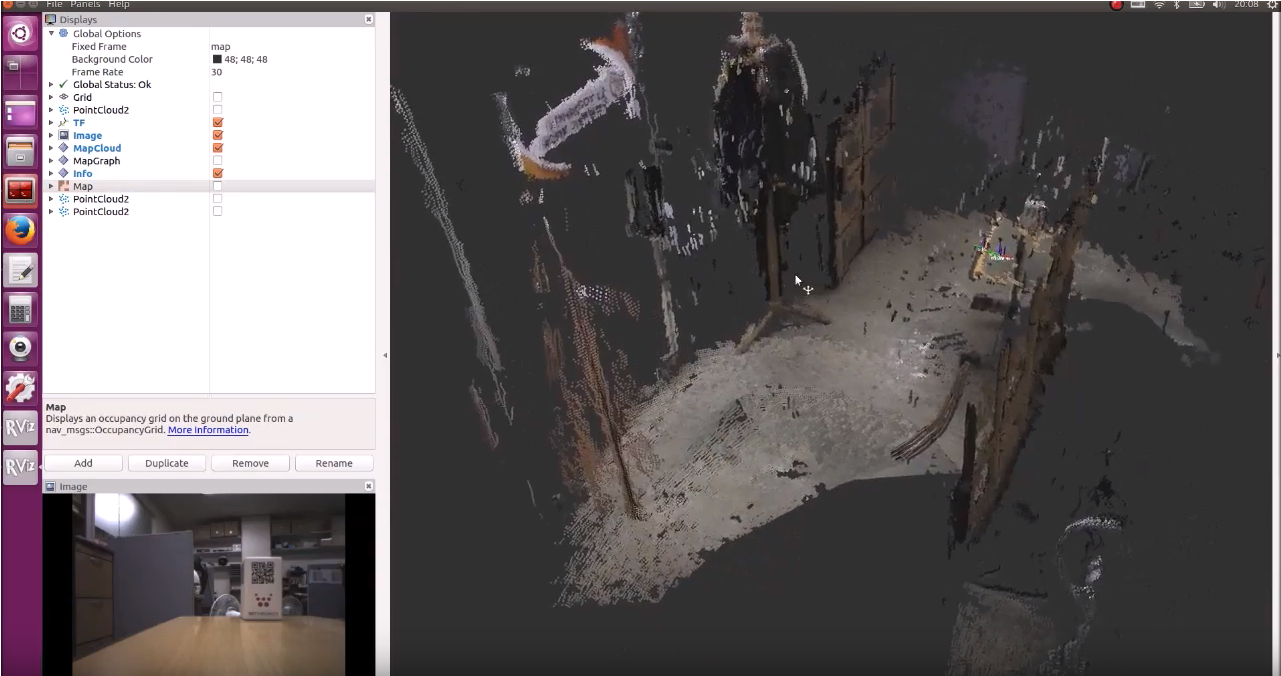
\includegraphics[width = 0.75\textwidth]{./Images/slam-map.jpg} 
\caption{A robot performing S.L.A.M in an environment and the 3D model created.}
\label{fig:slam}
\end{center}
\end{figure}

\subsection{How ARKit works}
\label{subsecARKit}
The easiest way to use ARKit is to use it through Xcode, which can be downloaded from the Mac App Store.
The coding language can be either Objective-C or Swift. We will be using Swift for all
examples.

ARKit works similar to SceneKit were a scene (which is basically a 3D environment in which nodes containing 3D models (geometry) can be rendered) is loaded at start up and interacted with.
An ARScene is contained inside an ARSCNView (AR Scene View) which also has an ARSession
that that manages the motion tracking and camera image processing. For an ARScene to work, it must have a running ARSession.
The session is started with configuration (ARConfiguration). This configuration can be of many kinds, the most common ones begin ARWorldTrackingConfiguration and ARFaceTrackingConfigurations. For this project, ARWorldTrackingConfiguration will be used since the face tracking one uses the front camera.

Below, an example of how to setup a configuration and running a session using Swift is given:

\begin{lstlisting}[language=swift]
func loadWorldTrackingConfiguration()
    {
        let configuration = ARWorldTrackingConfiguration()
        configuration.planeDetection = [.horizontal]

        // All the objects that are tracked is contained in the Objects folder
        guard let detectingObjects = ARReferenceObject.referenceObjects(inGroupNamed: "Objects", bundle: nil) else { return }
        configuration.detectionObjects = detectingObjects
        
        // Setting up tracking of images
        for imageURL in trackingImageURLs
        {
            guard let image: CGImage = UIImage(named: imageURL)?.cgImage else { return }
            let referenceImage = ARReferenceImage(image, orientation: CGImagePropertyOrientation.up, physicalWidth: 0.3)
            configuration.detectionImages.insert(referenceImage)
        }

        configuration.maximumNumberOfTrackedImages = trackingImageURLs.count
        
        // Running the sessoin with the configuration
        sceneView.session.run(configuration)
    }
\end{lstlisting}

But before a session can be started, an ARScene must exists and be loaded. The ARScene is a regular .scn file that has the starting nodes that together form the starting
environment the user will interact with. An example of how a scene like that looks like is shown in figure \ref{fig:3dsceneImage}.

\begin{figure}[hbtp]
\begin{center}
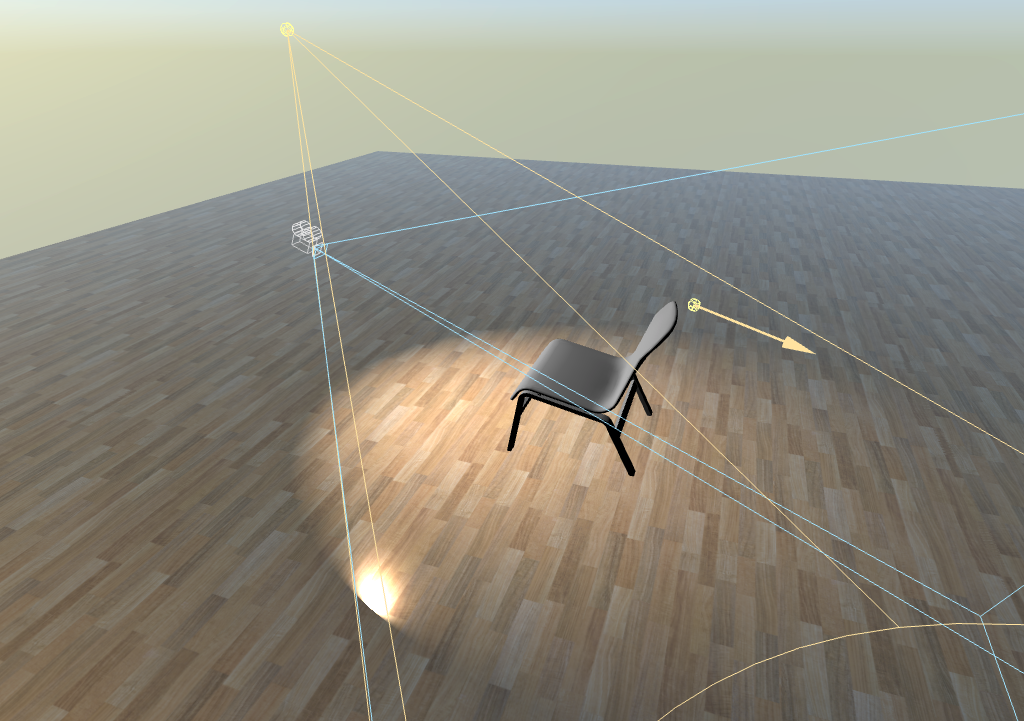
\includegraphics[width = 0.75\textwidth]{./Images/3dscene.jpg} 
\caption{An example of a 3D scene created in XCode with a camera, a plane, directional light and three geometry nodes.}
\label{fig:3dsceneImage}
\end{center}
\end{figure}

To load a scene, a new .scn file must be created in the art.scnassets folder and fetched like below.
\begin{lstlisting}[language=swift]
// Load the scene
let scene = SCNScene(named: "art.scnassets/world.scn")!        
sceneView.scene = scene
\end{lstlisting}

When ARScene detects objects, images, planes etc. it calls the renderer function. This function can be implemented by setting the ViewController to conform to the ARSCNViewDelegate. ARScene adds an anchor (ARAnchor) and a node (SCNNode) for the place where it detected it, and this can be used inside the function to render new nodes or other logic.

\begin{lstlisting}[language=swift]
func renderer(_ renderer: SCNSceneRenderer, didAdd node: SCNNode, for anchor: ARAnchor)
    {
    	    // If detected an object
        if let objectAnchor = anchor as? ARObjectAnchor
        {
        	   // Add some 3D text to the scene
            let objectName = objectAnchor.referenceObject.name!
            let textNode = GeometryFactory.makeText(text: objectName)
            node.addChildNode(textNode)
        }
        // If detected a plane
        else if let planeAnchor = anchor as? ARPlaneAnchor
        {
        // Add a plane geometry of the detected floor to the scene
        node.addChildNode(GeometryFactory.createPlane(planeAnchor: planeAnchor, metalDevice: metalDevice!))
            model.numberOfPlanesDetected += 1
        }
    }
\end{lstlisting}

If nodes need to be rendered outside of this function it can be done by accessing the
scenes root node.

\begin{lstlisting}[language=swift]
sceneView.scene.rootNode.addChildNode(node)
\end{lstlisting}


\newpage
\chapter{Neural Networks}
This chapter will focus on neural networks and how they were utilized for parts of this
report. First, some theoretical background surrounding neural networks in general, and then
more specifically, convolutional neural networks, is given in sections \ref{sec:NNwork}
and \ref{sec:CNN}.
Afterwards, the chapter goes more into how neural networks were tried and used during this project. Data collection and augmentation is described in sections \ref{sec:NNdata} and \ref{sec:NNaugment}. Further sections, \ref{sec:NNclassification} \& \ref{sec:NNtransfer}, describe how this data was used to train neural networks, with the latter section explaining an alternative to training a model from scratch. 
\section{How neural networks work}
\label{sec:NNwork}
There exists many different machine learning techniques out there today. Due to its high 
effectiveness and relevance, for this report we are going to focus on the highly popular 
method of artificial neural networks.
A variant, convolutional neural networks, is a proven method for working well with 
images and is therefore highly relevant for this project.

\subsection{Artificial neuron}
An artificial neuron is the simplest form of the neural network. It has a set of inputs and an output.
The artificial neuron first sums up all the input values, $x$, multiplied with the weight value, $w$.
After that it passes that sum through an activation function. This activation function can be everything from a simple $f(x)=x$ to the more complex sigmoid function, depending on the need. More on this in section \ref{subsec:activationfunctions}.

\begin{figure}[hbtp]
\begin{center}
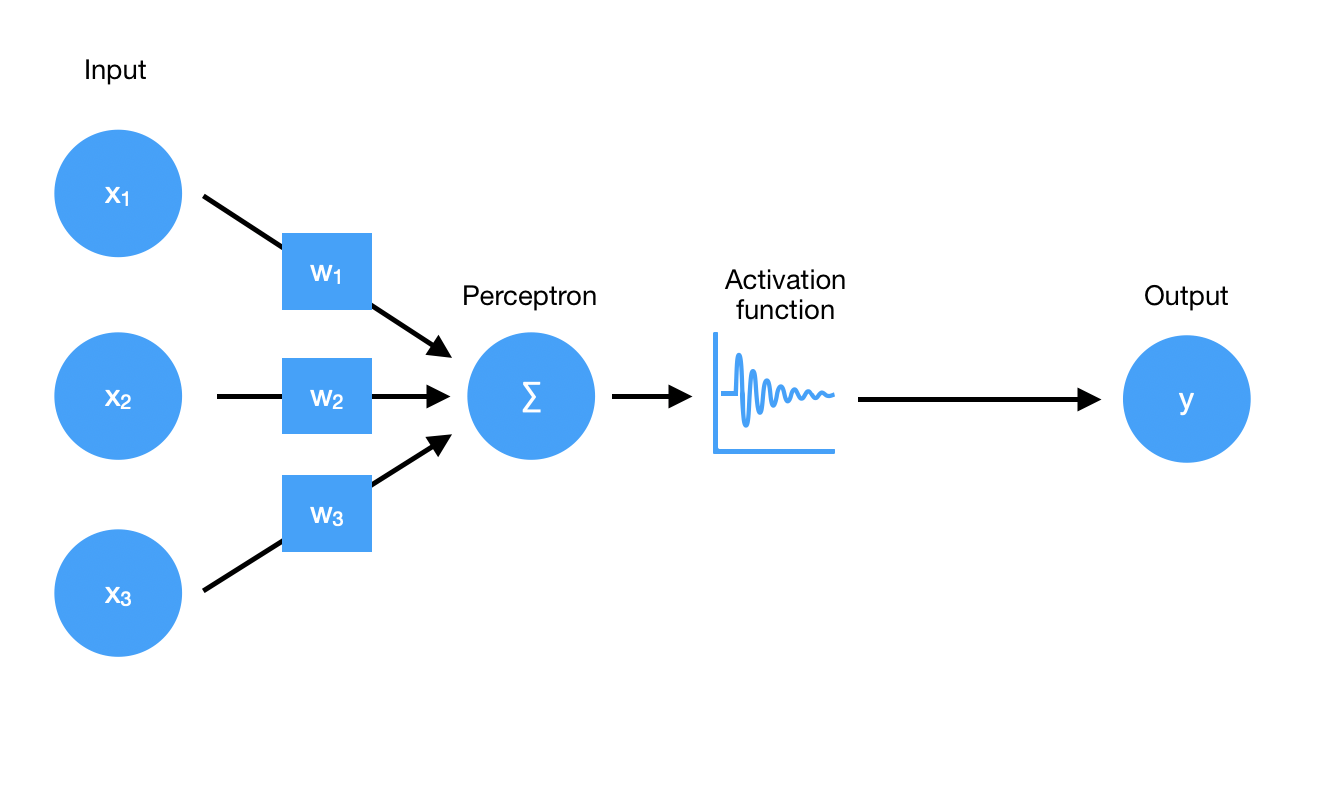
\includegraphics[width = 0.75\textwidth]{./Images/perceptron.jpg} 
\caption{An illustration of an artificial neuron, the simplest version of a neural network.}
\end{center}
\end{figure}

A bias also exists in every node which is not based on any input. The bias function in the artificial neuron is similar to what the $m$ in $y = kx + m$ does. It gives the function the ability to move up and down in the graph for more possibilities of splitting the data set. The bias is usually disregarded when illustrating the artificial neuron.

The artificial neuron only has the ability to draw a single line and thus is only able to split simple data sets.

The output of an artificial neuron is described by the following formula:

\[ y = b + \displaystyle\sum_{i=1}^{n} x_i \cdot w_i \]

\[y=f(b+\sum_{i=1}^n x_i\cdot w_i)\]

where $b$ is the bias value, $x$ is the input, $w$ is the weight for that input, $n$ is the number of inputs and $f(*)$ is the activation function.

\subsection{Activation functions}
\label{subsec:activationfunctions}
The activation function,  $ \phi (v_{i}) $ , takes the sum of all the inputs from a node as input and passes them through a function before giving an output. This is beneficial when for instance the output should be kept in a range between 0 and 1, or perhaps when negative values don't make sense.
Usually, activation functions are attributed to layers instead of individual nodes.

A few commonly used functions are \textbf{ReLu}, \textbf{Tanh}, \textbf{Sigmoid} and \textbf{Softmax}.

\textbf{ReLu} is described as
\[f(x) = max(0, x)\]
and is a good option when negative values should be ignored or don't make sense. 
It is also a good choice avoiding the net to become computationally heavy,
since it only outputs the same input value but sets all negative values to zero.
That is usually a good choice in larger networks with many neurons which can become
slow.

\textbf{Tanh} is the tangens hyperbolicus function and is used to output values either as -1 or 1 like a binary operator. Unlike a binary operator, tanh's derivative is always defined which makes back propagation possible.
Back propagation is described in section \ref{subSec:optimizers}

\textbf{Sigmoid} is described as 
\[\frac{e^x}{1+e^x}\]
and works like the Tanh function but keeps the values between 0 and 1 and sets y(0) = 0.5 instead.

\textbf{Softmax} is a little bit more complex. It takes a vector $v$ of dimension $n$ and turns it into a vector $\sigma(v)$ of the same dimension where $\displaystyle\sum_{i=1}^{n} \sigma_i(v) = 1 $ and each element value is between zero and one.

Each element in the array is described as below
\[ \sigma_i(v) = \frac{e^{v_i}}{\displaystyle\sum_{j=1}^{n} e^{v_k}} \]

This output is good for describing the probability for each element to be correct and is therefore commonly used
in the output layer.

\subsection{Calculating the loss}
When training the model, it will at first make a guess to what the right answer or value is based on the random initial weigh values. In the beginning, the model is usually mostly wrong and it is then important to know how wrong it was and in what direction it should go.

For this, the model uses a loss function to calculate that error. For different applications the loss function can be different.
One way to calculate the error, $E$, is to simply take the predicted value, $y_p$, and subtract it with the correct value, $y_c$.

\[E = y_p - y_c\]

Sometimes the sign of the error is not important. Then the absolute value can 
be calculated instead. $E = |y_p - y_c| $

Another approach is the \textbf{mean squared error} which squares the difference and takes the mean value over a few predictions. $n$ is the number of predictions.
\[E(n) = \frac{1}{n} \cdot \displaystyle\sum_{}^{n} (y_p - y_c)^{2} \]

\subsection{Optimizers}
\label{subSec:optimizers}
Once the error has been calculated, the network will make changes to itself to improve the performance by decreasing the error value. This is called backpropagation.
The principle behind backpropagation is to go backwards in the network from the output node and changing the weight values, $ \omega $.
The optimizers decide how the weights should change. \\

A popular method for minimizing the error is to use \textbf{Gradient Decent} which works
by, step by step, move in the negative direction that minimize the error.
The direction is determined by taking the derivative of the error function.
The new weight value is calculated accordingly. $\eta$ is a chosen parameter called the learning rate.

\[ \Delta \omega_{ik} = -\eta \frac{\delta E}{\delta \omega_{ik}} \]

\begin{center}
where the error function is
\end{center}

\[E = \frac{1}{N} \displaystyle\sum_{i=1}^{N} E(n) \]

\begin{center}
where N is the total number of neurons. This leads to
\end{center}

\[ \hat{\Delta\omega_{ik}} = \frac{1}{N}  \displaystyle\sum_{i=1}^{N} \Delta\omega_{ik}(n) \]

$ E(n) $ can be, for example, mean squared error mentioned above.
The most common form of gradient decent is called \textbf{Stochastic gradient decent}, SGD.
The difference is that SGD only evaluates on a small number of nodes/patterns, $P$ and updates all the weights from that observation.

\[ \hat{\Delta\omega_{ik}} = \frac{1}{P}  \displaystyle\sum_{i=1}^{P} \Delta\omega_{ik}(p) \]

\textbf{Adam}\cite{adamoptimizer}, short for Adaptive moment estimation, is another optimizer which is quite popular.
The reason is because it has been proven to be a very effective algorithm in many different use cases.

Adam is a kind of combination of using \textbf{RMSPROP}\cite{rmsprop} and SGD with momentum.
Without going into too much detail, SGD with momentum keeps track of which direction the the improvement is in and keeps the improvement going in that same way. The optimisation goes faster when the previous direction is the same and slower when they are different. Almost like a rolling ball that gains speed as it is rolling down hill.
RMSPROP does something similar and uses a running average of each weight value and the previous values importance can be controlled with a parameter. It also only uses the sign of the direction and not its value. Also RMSPROP has individual weights.

Adam keeps a running average of both the past gradients and the squared past gradients.
The full mathematical description of Adam is given by the formula below where
$t$ is a time iteration index.

\[ \omega_i (t+1) = \omega_i(t) - \eta \frac{m_i}{\sqrt{v_i} + \epsilon} \]

where

\[ m_i (t+1) = \beta_1m_i(t) + (1 - \beta_1) \frac{ \delta E(t) }{\delta\omega_i} \]

\[ v_i (t+1) = \beta_2v_i(t) + (1 - \beta_2) (\frac{ \delta E(t) }{\delta\omega_i})^2 \]

and $ \eta, \beta_1 $ and $ \beta_2 $ are adjustable parameters and $ \epsilon $ a small value to keep the equation from dividing by zero.\\

There are a lot of other optimizers such as \textbf{Adagrad}, \textbf{Adadelta}, 
\textbf{Nadam} \cite{optimizers}. They all have their own advantage and use-cases.
We won't go into further details about them.

\subsection{Layers}

\begin{figure}[hbtp]
\begin{center}
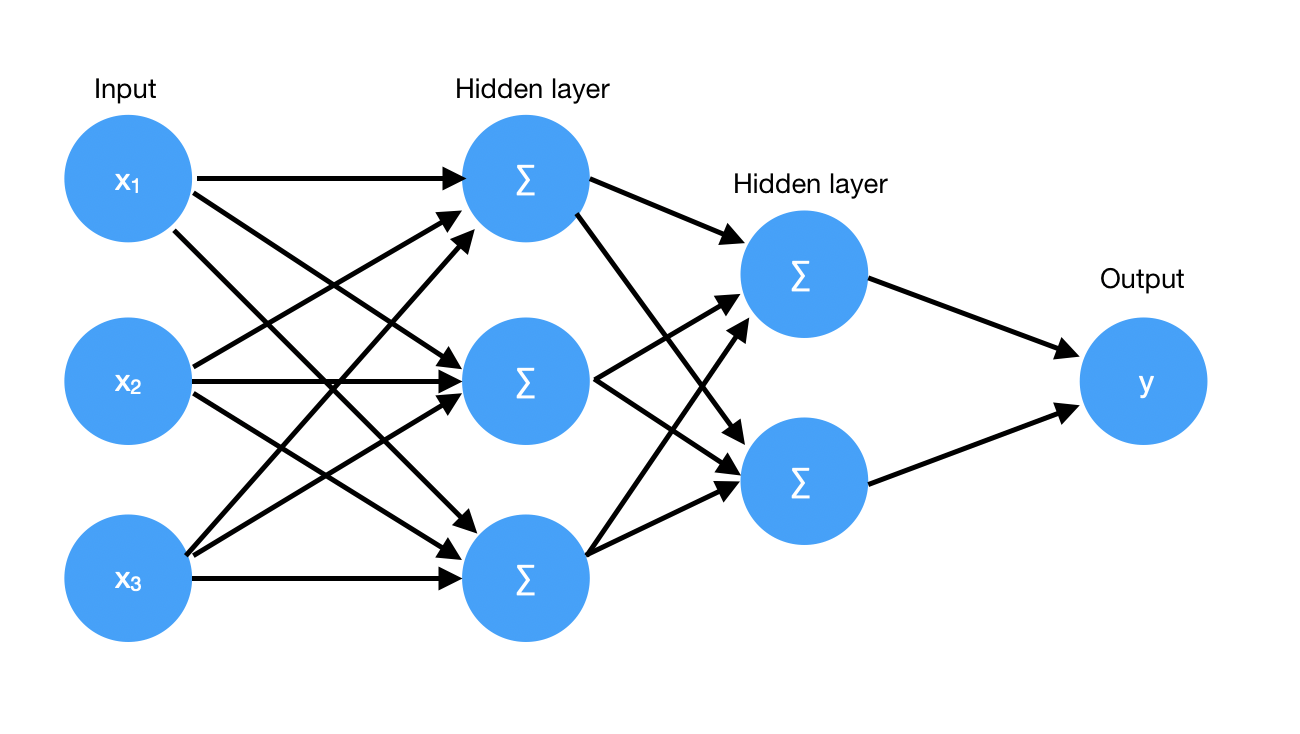
\includegraphics[width = 1.0\textwidth]{./Images/fully_connected.jpg} 
\caption{Two fully connected layers. One with 3 neurons and one with 2 neurons.}
\label{fig:layers}
\end{center}
\end{figure}

With more layers and more neurons the networks parameters and complexity begins to grow. So does also the training time, size of the model and the cost for doing predictions. 
Thus, these networks are capable of describing much more complex data sets. But as a result of that, the risk of overfitting, the act of describing the training data set too well so that new data sets will not get recognized, becomes much greater.
That is why a complex network is not always wanted.
In figure \ref{fig:layers} an example is given of how a network with many layers might look.

\subsection{Overfitting}
\label{overfitting}
When training a neural net, one needs to be careful not to train the model too much or overfitting is likely to happen.
Overfitting is when a model gets really good at predicting the data that it is training on but fails to predict accurately on new data.
This is because it starts to pick up too much on detail or in some instances even noise.
For this reason it fails to pick up the general trends, which is more valuable.
An illustration is given i figure \ref{fig:overfitting}.

\begin{figure}[hbtp]
\begin{center}
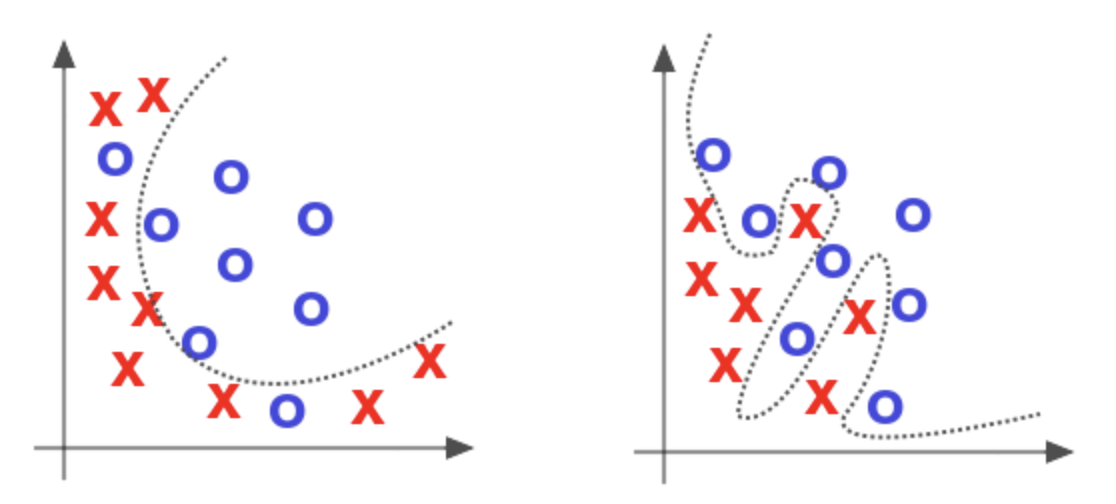
\includegraphics[width = 1.0\textwidth]{./Images/overfitting.jpg} 
\caption{Overfitting of a dataset. On the left is a generalized trained model and on the right is an overtrained model. Image taken from OReilly.com \cite{overfitting}.}
\label{fig:overfitting}
\end{center}
\end{figure}

There are a few methods that can help handle the problem of overfitting. They usually involve trying to limit the size of a small amount of weights.
The hypothesis behind this is that if a weight is much larger than the rest it also has much more influence over the final prediction. That way, a small detail in the data can have much more influence than the general trend.

One way to do this is to cut random connections between layers during epochs, usually by specifying a certain amount that is going to be cut.
This way, the model is not relying on a small number of nodes to make the correct predictions. This method is called \textbf{dropout} \cite{dropout}.

Another way is to introduce random noise on a layer during training. This works because if a node with a large weight receives noise, it will be heavily amplified and probably give a false prediction.
When doing this, Gaussian noise is usually implemented, which is basically random noise with a gaussian distribution.

To force the model to keep weights small, one way is to add a penalty to the loss for every weight based on its size. 
This is called weight regularisation and is widely used and exists in two forms, L1 and L2.
L1 simply adds the weights size multiplied with an L1 term that is chosen by the designer.
The other, L2, is to do the same but in this case square that value. This has the effect of making values over 1 even bigger and values less than 1 smaller.
In that way, it doesn't affect the loss as much as L1 when not being overtrained. L2 is also called weight decay and is the more common method of the two.

Another way to keep the values small is to normalize the input to every layer and set the mean to 0 and variance to 1. In Tensorflow, this can be done with the BatchNormalization layer \cite{batchnormalization}.

One important thing to point out is that all these methods mentioned so far are only active during training and is not doing anything when making real predictions.

If lots of training data exists, the ensemble technique could be a good way to go. This technique divides the training data into smaller sets and trains a model for every data set.
The final prediction is then an average of the predictions of all the models. This technique works because if the model is highly overtrained in a certain direction, chances are that the other networks will drown out this result by the many other models.

It is kind of like when someone has an off pitch in a big choir. If there are many other singers, this off-pitch will not be noticed very much.

The final technique is called early stopping and is based on validating the model after every 
epoch and stopping the training when the validation loss, or some other criteria, is not 
improving anymore. A graph showing when to do early stopping is given in figure \ref{fig:earlystopping}.

\begin{figure}[hbtp]
\begin{center}
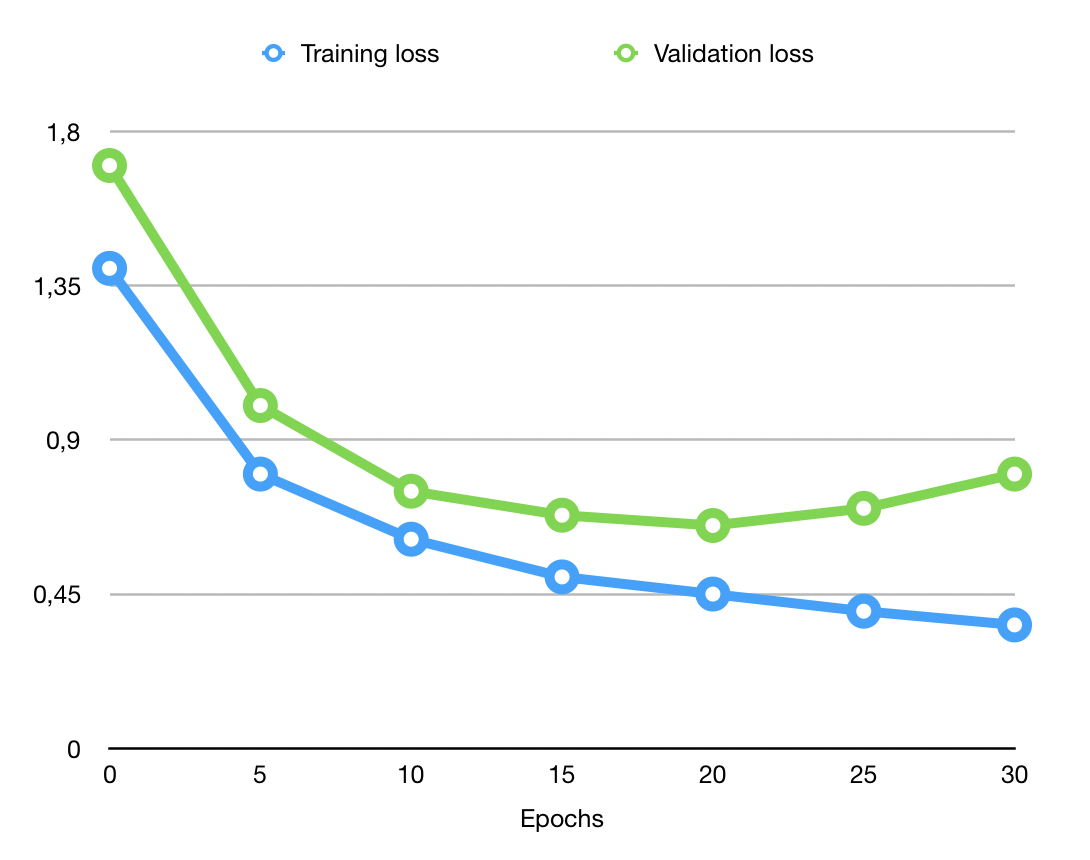
\includegraphics[width = 0.75\textwidth]{./Images/early_stop.jpg} 
\caption{A graph showing when to do an early stop. The graph shows the total loss over trained epochs. Notice that the validation starts to increase again somewhere after epoch 20.}
\label{fig:earlystopping}
\end{center}
\end{figure}

 \section{Convolutional Neural Networks}
 \label{sec:CNN}
Convolutional neural networks, CNN, have been used for quite some time when it comes to deep learning and their capabilities are rather astounding, as proved by Krizhevsky et al \cite{NIPS2012_4824}.  They use layers which perform convolutions, hence it's name.  The input to a convolutional network are either 2D or 3D tensors, where the 3D alternative usually has color channels along the third dimension. Use of convolutional neural networks in image recognition  can be practical for several reasons, e.g., it can tell of spatial relationships in an image. This section has been written with reference to V. Dumolin et al \cite{convArit}. Figure \ref{fig:cnn} shows an example of how a CNN may look.
 
 \begin{figure}[hbtp]
\begin{center}
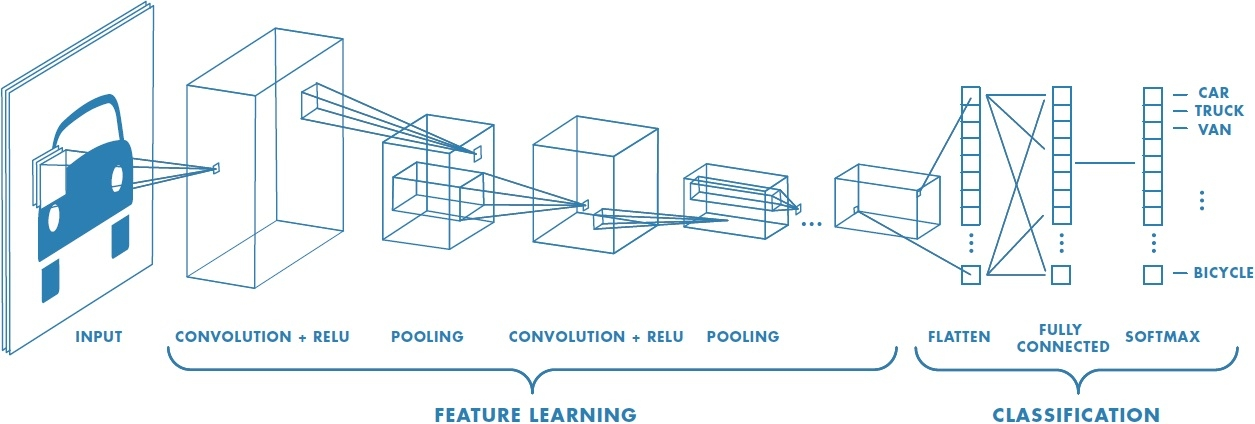
\includegraphics[width = 0.9\textwidth]{./Images/convNetwork.jpg}
\caption{Image shows the flow of a convolutional neural network from left to right. Several convolutions as well as pooling functions are done in order on the input image. The last feature map is then flattened to fit into the hidden layers, to then be classified with a softmax function. Image taken from \cite{cnnImage}.}
\label{fig:cnn}
\end{center}
\end{figure}
 
A convolutional layer performs the mathematical operation \textit{convolution} on the input tensor, which can be presented as an image. A convolutional filter, or kernel, of size $k \cdot l$ slides across the input. The kernel consist of weights in each element. These weights are found during the training process of the network. As the kernel is slides across the image, the dot product of the weights of the kernel and the pixels the the kernel is above, is calculated as the output. Afterwards, a new image containing all of the produced dot products is formed.

Padding on the input can be used to account for values when the kernel is outside the input. Use of padding have an impact on the output size after the convolutional layer. Stride can also be used, which tells how much the kernel translates along an axis;  increased stride leads to subsampling. Since changes of parameters in one axis do not affect outcome in another axis it simplifies explaining CNNs by having the parameter values being the same along both axes. The more convolutional layers used in a network, the more complex shapes are detected. First layers may detect edges and corners, whereas, later layers may find features representing, for example, a car or a dog. A common addition to the layers is an activation function, commonly ReLU (which is described in section \ref{subsec:activationfunctions}). This gives faster training by only allowing for positive weights to pass the layer.

 The common types of padding is \textit{no zero}, \textit{same} and \textit{full}; examples seen in figure \ref{fig:padding}. No Zero padding involves having no padding outside of the input. This means that the kernel never goes outside of the actual image, once a side of the kernel hits the side of the input it jumps down to the next line (if stride is 1). 
 
 Same padding is used when one desires the output size of the layer to be the same as the input size. This is achieved by having a padding $p$ be $ p = \floor{\frac{k}{2}} $ for any odd kernel size $k$.
  
 With full padding one actually makes the output size larger than the input, by fully utilizing every possible combination of the kernel and the input image. This is accomplished  by having the padding $p $ be $p = k - 1$ for any kernel size $k$. 
 
 
 \begin{figure}[hbtp]
\begin{center}
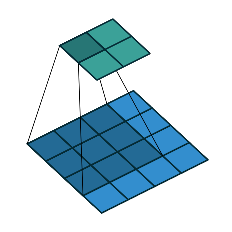
\includegraphics[width = 0.3\textwidth]{./Images/noPad.png}
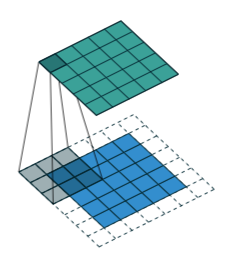
\includegraphics[width = 0.3\textwidth]{./Images/samePad.png}
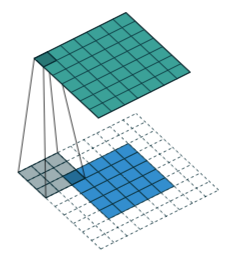
\includegraphics[width = 0.3\textwidth]{./Images/fullPad.png} 
\caption{Different examples of padding. Grid in green is the output, grid in blue is the input, and area in shadow is the current area where the kernel is currently at. Leftmost image shows a no zero padding being used. Here the kernel size is $k = 3$, input size is $i = 4$ and the output size is  $o = 2$, i.e., smaller than input.  In the middle image same padding is used; output size is the same as input size $o = i = 5$. In the rightmost image full padding is used. Here a bigger output size than the input size is produced, $o = 7, i = 5$. Images taken from \cite{convArit}}
\label{fig:padding}
\end{center}
\end{figure}
 
 
 Another useful feature used in a lot of convolutional neural networks is pooling. Pooling layers are somewhat similar to convolutional layers in that they use a sliding window which performs an operation on the contents of the window and outputs a new value. However, the difference is that they use other functions instead of linear addition. Two common pooling functions are \textit{max pooling}, where the output is the largest value within the window, and \textit{average pooling}, where the output is the average of the components within the window.  Pooling is commonly done do reduce the size of the input. Figure \ref{fig:pooling} shows example of pooling being used.
 
 \begin{figure}[hbtp]
\begin{center}
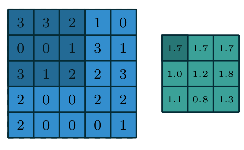
\includegraphics[width = 0.45\textwidth]{./Images/avgPool.png}
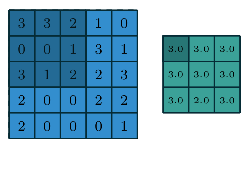
\includegraphics[width = 0.45\textwidth]{./Images/maxPool.png}
\caption{Examples of two types of pooling. Blue grid represents input, green grid represents the output, and the shaded area is where the sliding window is located. The left image shows the use of average pooling, while the right one shows the use of max pooling.
Images taken from \cite{convArit}}
\label{fig:pooling}
\end{center}
\end{figure} 
 
When a classification is to be done in the CNN, the shape needs to be shifted to an array. This is done after the last pooling layer or convolutional layer. This array can then be passed into a hidden layer for classification.


\section{Collecting data}
\label{sec:NNdata}
When working with machine learning, big sets of data is often required for a good resulting model.
A problem with this is that it can be tricky to obtain such a large data set because it usually also requires
labels with that data to be manually put in. These labels will be used by the neural network to, during training, check if
the predicted value is correct or not.

In this project the data is sets of images of different furniture parts. These images did not exist anywhere online, so they had to be collected by taking lots of photos. The photos contained the part in different background and from different angles. Table \ref{table:imageclassnumbers} shows how many images of each class we had. The backgrounds were mostly of typical office surroundings, although there were exceptions (example is shown in figure \ref{fig:exampleCutout}). All the photos were then resized to 256x256 pixels.
The reason for choosing a square size is because when rotating them
(this will be useful later on when augmenting data in section \ref{sec:NNaugment}) 
the images will not have any black bars on the sides nor be stretched.

\begin{table}[h]
\centering
\begin{tabular}{ |c|c| } 
 \hline
 Class &  Number of images  \\ 
 \hline
 Leg piece & 203 \\ 
 \hline
 Bridge piece & 210 \\ 
  \hline
 Seat & 216 \\ 
 \hline
\end{tabular}
\caption{Table showing how many images of each class we had.}
\label{table:imageclassnumbers}
\end{table}

For the first furniture Nolmyra, there were only 3 unique parts (excluding screws and similar parts). Therefore the model was trained to recognize 4 things; the different parts and an unknown object. The unknown label was because the object detection algorithm could detect other objects and it is then unwanted that those objects be mistaken for furniture parts. This could of course also be done by setting a threshold on the confidence value, i.e., if the model gives a confidence value under 0.8 it discards it as being an unknown object. The problem with this type is that it is much harder to distinguish parts from unknown objects. This is due to that the best model is the one that can give a close to 100\% confidence value on every prediction.

For this reason, photos of random objects were also added to the data set. Most of these photos were taken by ourselves, but some were also collected from the web. The images were placed in folders with a specific item which meant labelling them became much simpler. Just put all the images containing a certain part in the same folder.

Training a model usually requires hundreds of thousands or even millions of photos. That much data is hard to get and would take a lot of time to obtain Going around the office to snap that many photos is almost unthinkable.
However, there are other options which will be explained in the next section.

\begin{figure}[hbtp]
\begin{center}
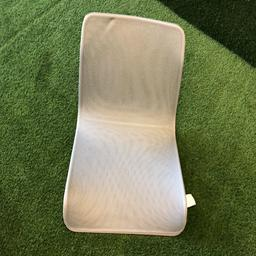
\includegraphics[width = 0.3\textwidth]{./Images/image_31.jpg}
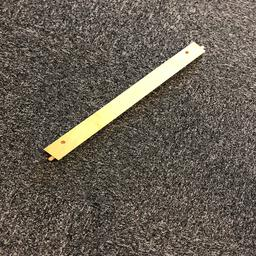
\includegraphics[width = 0.3\textwidth]{./Images/image_133.jpg}

\includegraphics[width = 0.3\textwidth]{./Images/image_136.jpg}
\caption{Images showing different samples of training data used for training the model. From left to right: seat, bridge piece, leg piece.}
\label{fig:exampleData}
\end{center}
\end{figure}

\section{Augmenting data}
\label{sec:NNaugment}
Instead of training on only original images, some images can be created from other images by for example rotating, flipping, changing brightness, saturation, contrast etc.  This will essentially be an image of the same object, but the data will look different, thus giving the model more relevant data to train on, see figure \ref{fig:exampleArtificial}.
When doing this it is important to keep in mind that the augmented data should be relevant to real situations.
Creating data with only the blue color band when the real situations are only in daylight makes no sense.

\begin{figure}[hbtp]
\begin{center}
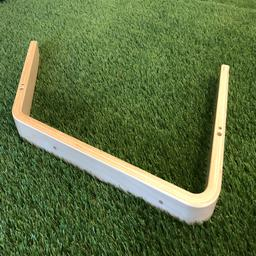
\includegraphics[width = 0.3\textwidth]{./Images/image_15-1.jpg}
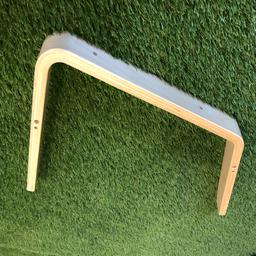
\includegraphics[width = 0.3\textwidth]{./Images/image_15-3.jpg}
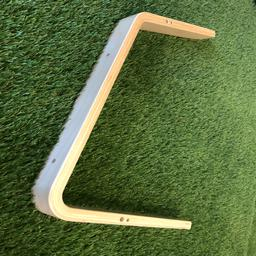
\includegraphics[width = 0.3\textwidth]{./Images/image_15-4.jpg}
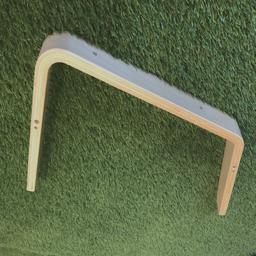
\includegraphics[width = 0.3\textwidth]{./Images/image_15-9.jpg}
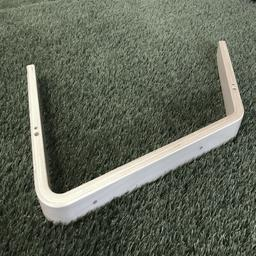
\includegraphics[width = 0.3\textwidth]{./Images/image_15-11.jpg}
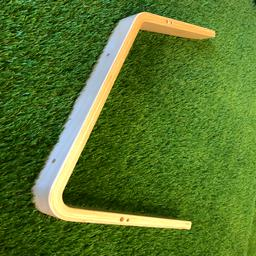
\includegraphics[width = 0.3\textwidth]{./Images/image_15-12.jpg}
\caption{Images showing some resulting images from augmentation. Top left image shows the original image. Top middle image shows the result after rotating $180$ degrees. Top right image shows result after rotating $-90$ degrees. Bottom left image show result after  reducing the contrast with by $30\%$. Bottom middle image shows result after reducing color balance by $70\%$. Bottom right image shows result after increasing color balance by $60\%$.}
\label{fig:exampleArtificial}
\end{center}
\end{figure}

Furthermore, images of objects of interest can be cut out and pasted into random environments to create even more data, see figure \ref{fig:exampleCutout}.
The idea of this is to try and make the model understand that the focus should be on the furniture part and the background environment is irrelevant. While doing this, even though the parts could be cut into totally random environments we tried to focus on pasting them into relevant spaces like office floors or carpets.
In our project, this gave a good result as it increased the test accuracy by 8\%.

\begin{figure}[hbtp]
\begin{center}
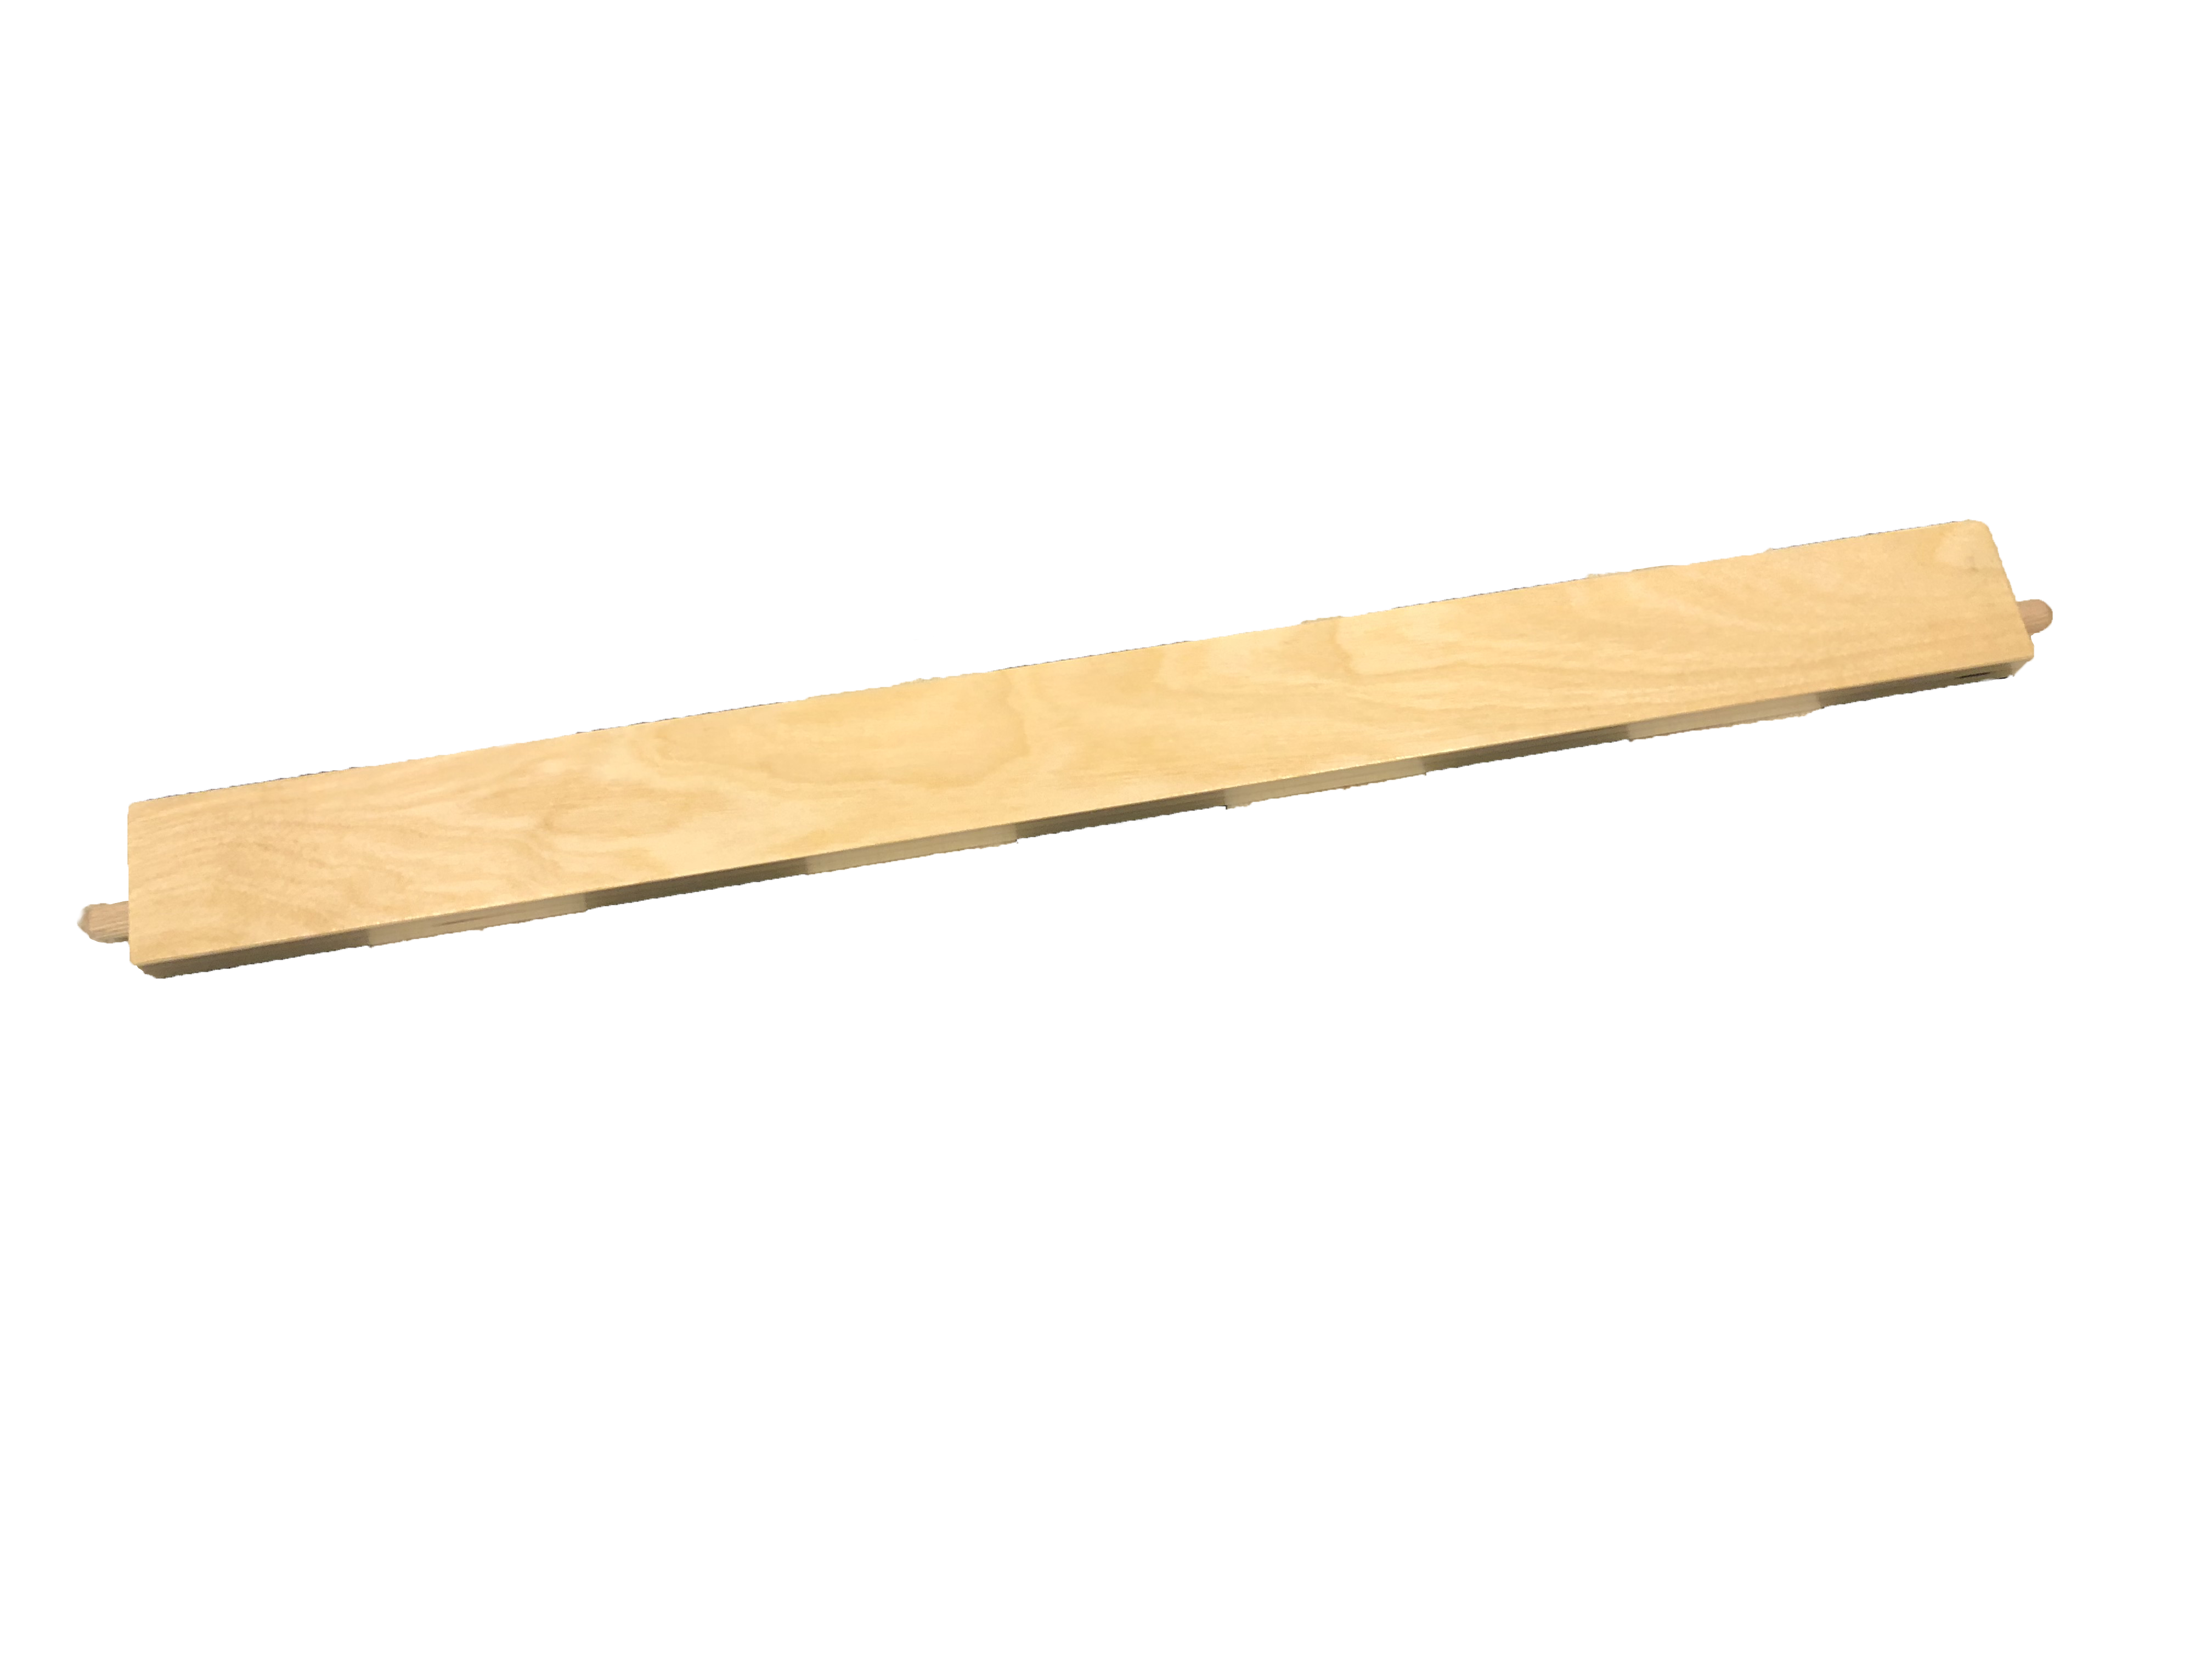
\includegraphics[width = 0.3\textwidth]{./Images/image_13.jpg}
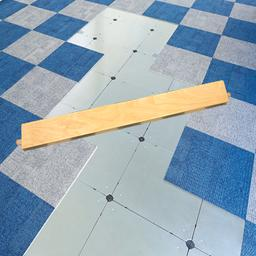
\includegraphics[width = 0.3\textwidth]{./Images/image_86.jpg}
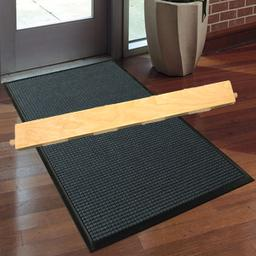
\includegraphics[width = 0.3\textwidth]{./Images/image_107.jpg}
\caption{Images showing how cutouts of images were utilized. Leftmost image shows a cutout of one of the furniture parts. The other two images show the result after they were pasted in to different environments to artificially increase training data.}
\label{fig:exampleCutout}
\end{center}
\end{figure}


Doing this by hand can still be very time consuming, so automating this process as far as possible is recommended.

\section{Image classification}
\label{sec:NNclassification}
Designing a neural network for the image classification is not the easiest task and much
work consists of trying things and making intelligent guesses.
As stated in the section about data collection we had 4 different classes to classify,
which means that a test accuracy of over 25\% would be significant. We were aiming for
somewhere above or around 90\% with a relatively small amount of data.

We started out with many convolutional layers layered with pooling layers and a few dense
layers at the end. The final layer had four nodes and softmax activation functions to give a
classification probability between four classes.
The activation functions of the other layers were set to ReLu since they are the fastest
and preferred for larger nets. Tanh was also tried but with no success.

SGD with momentum as an optimizer was tested but was changed to Adam
quite early on since it had better performance.
Only linear optimizers were considered because non-linear optimizers take a lot of
computing power and are usually only recommended for small networks.

We went back and forth with trying different mixes of kernel sizes, amounts of convolutional
layers, insertion of pooling layers on different places, stride sizes, amount of dense layers
and how many nodes they had.

When training the models, overfitting was a big problem from the start. The tested methods
for combating this was dropouts with different values, L2 weight regularisation,
batch normalization and reducing the number of weights.

It was hard to reduce the number of weights as the evaluation usually converged around 25\%
whenever it was tried.
When using the dropout method a value of 50\% with a minimum of 64 nodes in the layer
reduced overfitting most effectively. That, with a combination of weight regularisation and batch 
normalization gave good results. Figure \ref{fig:imageclassification} shows how overfitting was avoided.

Gaussian Noise gave very good results, but was unfortunately not possible to be 
converted from the model format generated in keras, to the mlmodel format that is required for Xcode.

The most important thing to mention is the difference the amount of photos we had and how they
were taken. Adding more photos made a huge difference to the test evaluation score.
After having added 50 more images per class with a library of 600 images the test score increased
from \textbf{80.55\%} to \textbf{83.45\%} in accuracy. \\

When finally testing the model we made a mistake by not separating the training data and test data.
Since we shuffled our data before splitting it up into two parts, some augmented data got into the
test set. The model had already trained on the original image and it was similar enough to
give unrealistic good results of 99.52\%. This was finally fixed by splitting up the test and train data 
into separate folders. Figure \ref{fig:augmentedtestdata} shows the printed graph from one of those
training sessions.

\begin{figure}[!hbtp]
\begin{center}
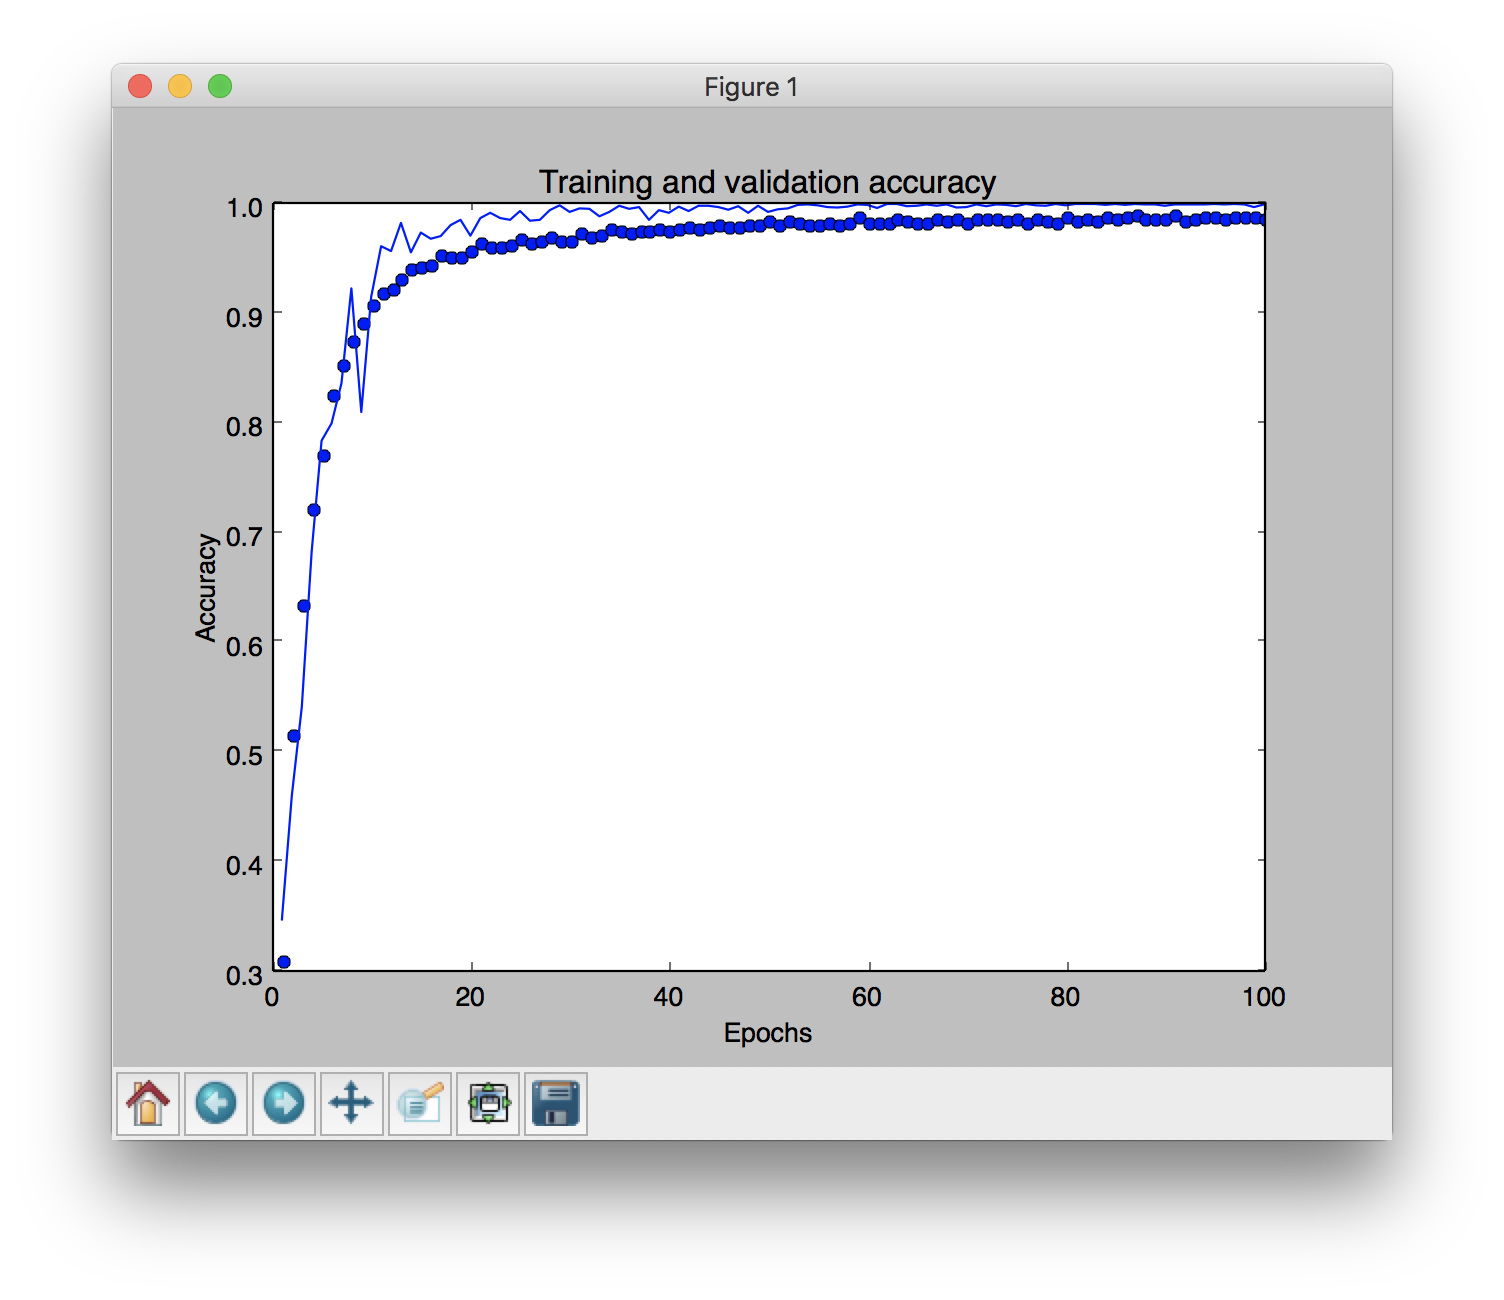
\includegraphics[width = 0.5\textwidth]{./Images/augmentedtestdata}
\caption{Test and train accuracy over a 100 epochs. The performance seems much better than it actually is.}
\label{fig:augmentedtestdata}
\end{center}
\end{figure}

\begin{figure}[!hbtp]
\begin{center}
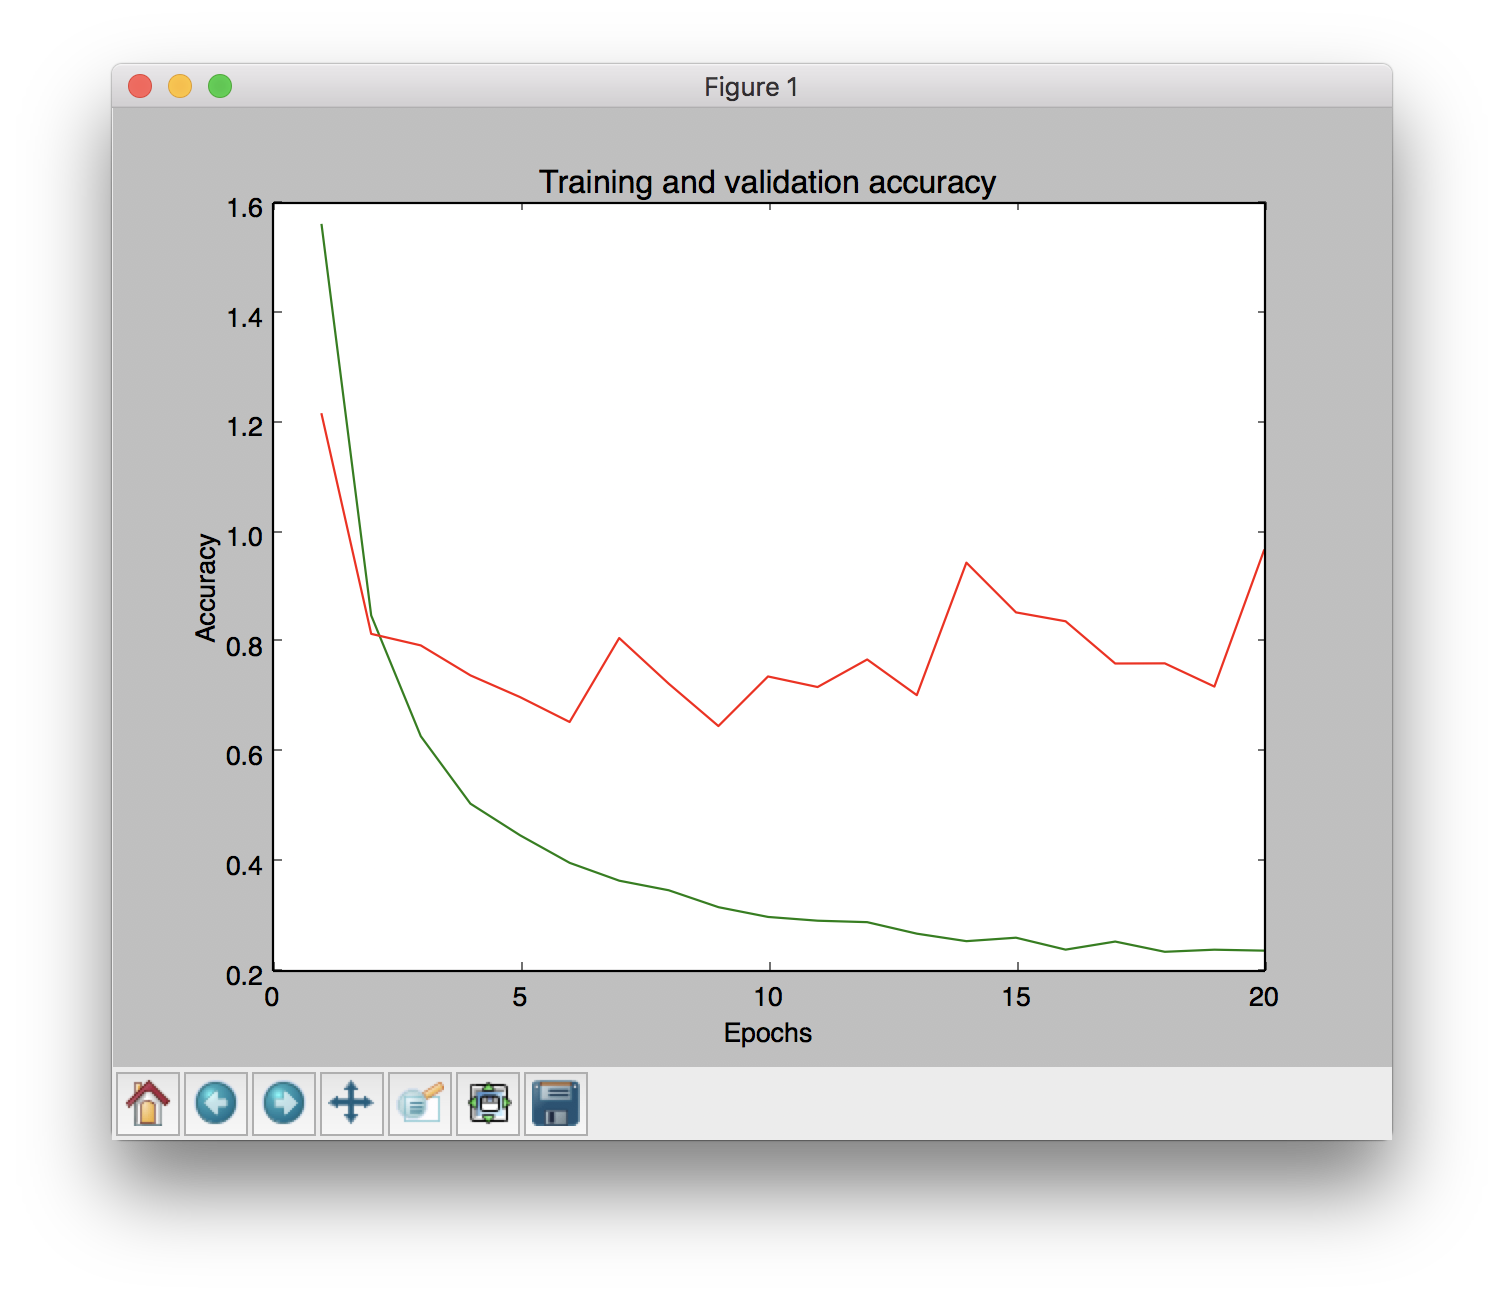
\includegraphics[width = 0.45\textwidth]{./Images/imageclassification1}
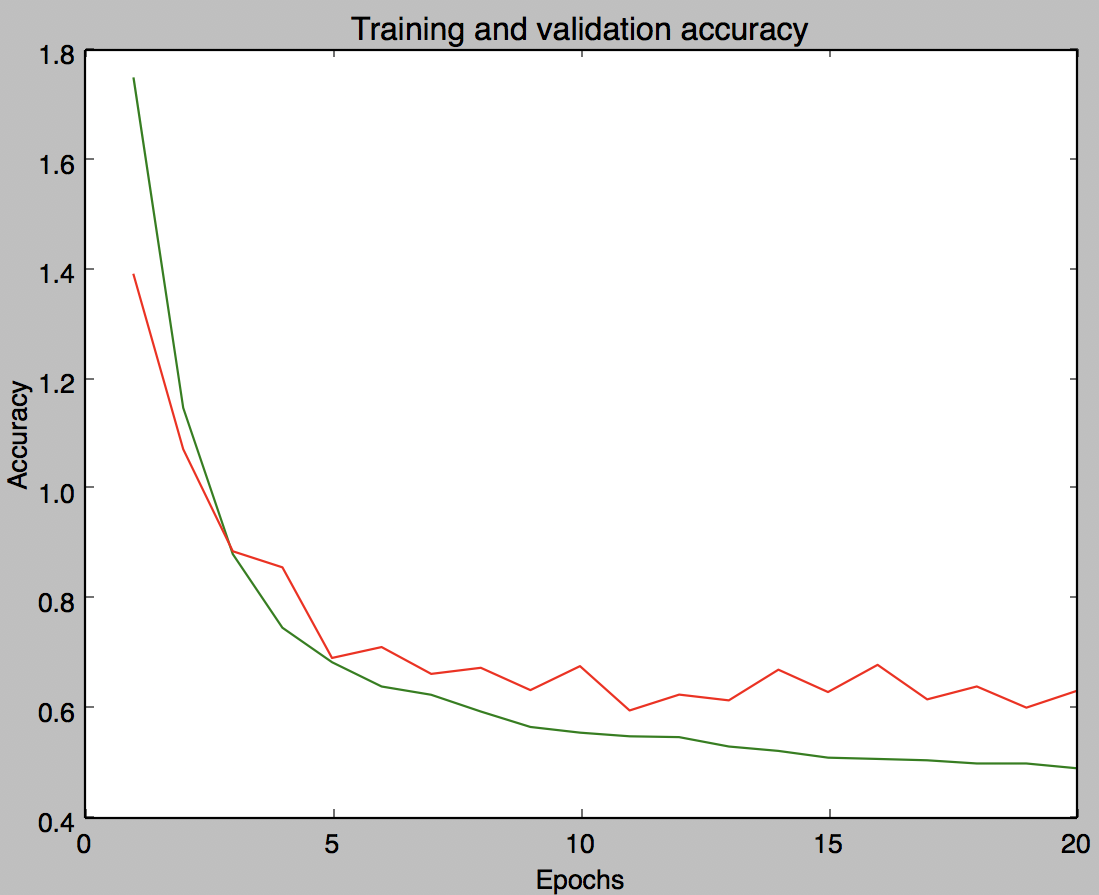
\includegraphics[width = 0.45\textwidth]{./Images/imageclassification2}
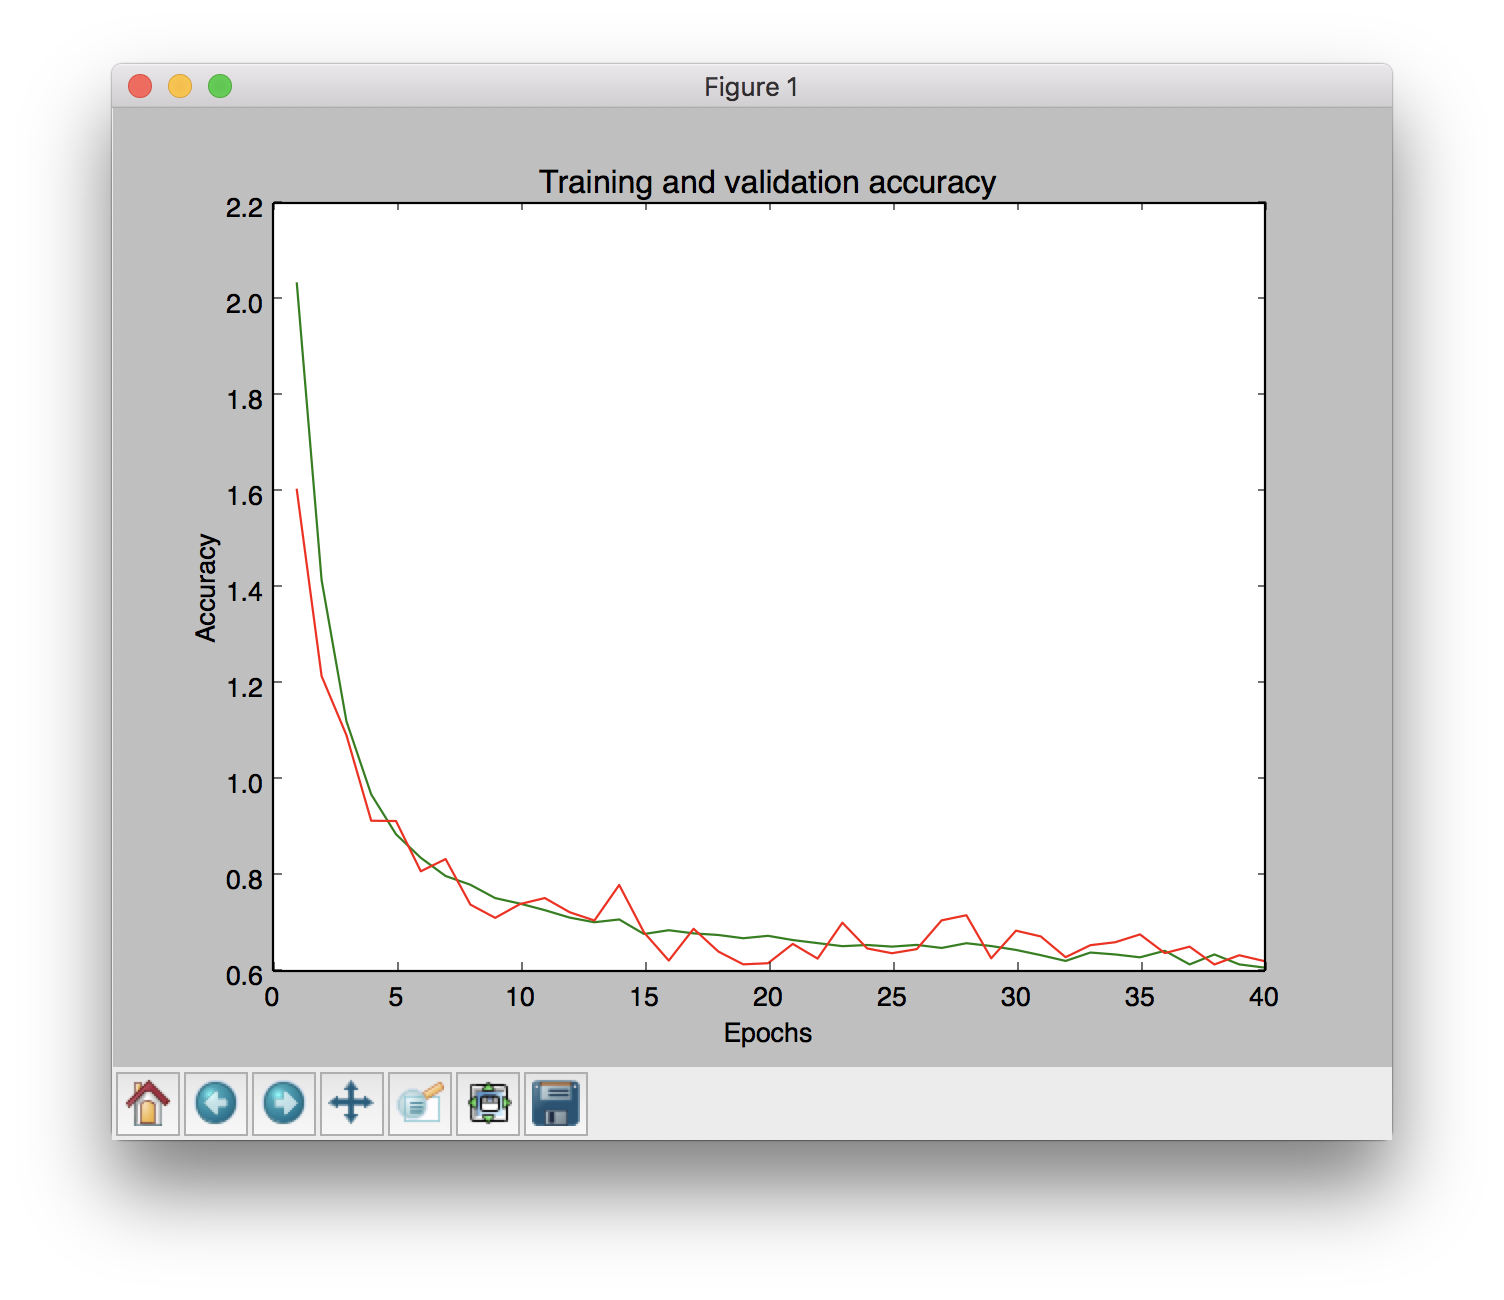
\includegraphics[width = 0.45\textwidth]{./Images/imageclassification3}
\caption{Images shows the result from introducing weight regularisation and dropout to a model. The graphs show the training loss (green) and evaluation loss (red). The upper left image shows the training without any dropout or weight regularisation. The upper right image shows the training with dropout implemented. The bottom image shows the training with dropout and weight regularisation implemented.}
\label{fig:imageclassification}
\end{center}
\end{figure}

As shown in the code in appendix B.1., early stopping was also finally implemented with a callback to save the
highest performing model at the end of the process.

The network that proved to be the best performing network (\textbf{92.25\%} accuracy) had the configuration shown in appendix B.2.

A model with many convolutional layers and a few dense layers at the end gave the best
results. A larger network could have been implemented and tests as well but
since the model size would grow more and training time would increase drastically,
we didn't increase it further.

\section{Transfer Learning}
\label{sec:NNtransfer}
% Write about how we went about in order to insert Transfer Learning into the mix. 
After trial of designing the network from scratch, it was decided to try and make use of 
pre-trained networks and then retrain them for another purpose. Models trained on 
imageNet \cite{imageNet} were chosen since that source domain is similar to this target 
domain. The models with their respective weights were loaded, without their fully 
connected layer. The top layer's weights were then frozen at different stages, and new 
fully connected layers were added on top, and new classifiers were trained. 
Several different models were tried, including ResNet50, InceptionV3 and VGG16, 
which where all integrated in Keras to start with.

The code shown in appendix B.3. shows how to load the VGG16 network which has weights that has been pretrained on imageNet. The fully connected layer is then removed and instead a custom top layer is added to be trained.

The best result  that was achieved for each of the models using this method is listed in
 table \ref{table:transferLearning}. It shows that using InceptionV3 model with pretrained
 weights gave the best result. However, a few factors, such as, where the models were
 frozen, how adding and removing layers, has most likely affected the results. As can be
 seen from using ResNet, the best model achieved 25\% accuracy, which is the same as making a guess, seeing as there are only four possible classes. These models could, and would most like have been, improved if it was not decided to take a new approach to the problem, which is described further in section \ref{sec:ODresults}.

\begin{table}[h]
\centering
\begin{tabular}{ |c|c| } 
 \hline
 Pretrained model used &  Best achieved accuracy  \\ 
 \hline
 VGG16 & 70.8\%. \\ 
 \hline
 ResNet & 25.0\% \\ 
  \hline
 InceptionV3 & 72.9\% \\ 
 \hline
\end{tabular}
\caption{Results from doing transfer learning .}
\label{table:transferLearning}
\end{table}


\newpage
\chapter{Object Detection}
At this point of the project process, a machine learning model capable of decently 
classifying which of the furniture parts were in the image existed. However, when using the 
planned application, it is very likely that there are several parts within the same frame. 
Hence, a method of localizing where an object was located was highly sought after. The idea 
was to find such a method, segmenting out the areas containing an object, and then use these  
areas as input images for to the machine learning model.

In this chapter, a few of the methods for object detection that were tried is explained, even though none of them ended up being viable in the end.
  
\section{Testing Object Scanning with ARKit2}
\label{sec:ODscanning}
Apple's ARKit2 has a feature where it can detect scanned 3D objects. For scanning, they have developed an app that can be downloaded from their website. \cite{ARScanning}
After the scanning is complete the app lets you export the model to then include it in your ARKit2 project. Once in the project it is simply imported into the ARWorldTrackingConfiguration like shown below. (The models are kept inside the Assets.xcassets catalogue in a folder called 'Objects').

\begin{lstlisting}[language=swift]
let configuration = ARWorldTrackingConfiguration()
guard let detectingObjects = ARReferenceObject.referenceObjects(inGroupNamed: "Objects", bundle: nil) else { return }
configuration.detectionObjects = detectingObjects
\end{lstlisting}

\begin{figure}[hbtp]
\begin{center}
\includegraphics[width = 0.32\textwidth]{./Images/3dscanning1.png}
\includegraphics[width = 0.32\textwidth]{./Images/3dscanning2.png}
\includegraphics[width = 0.32\textwidth]{./Images/3dscanning3.png} 
\caption{3D Scanning using Apple's app. On the left, the bounding box is defined so that no reference points from other objects are included. In the middle, the object is scanned by aiming the camera around the object at all angles. On the right the created model is tested. In this case, the object is detected after 0.4 seconds.}
\end{center}
\end{figure}

Once imported into our project we were able to test the performance of recognizing and tracking three pieces of our furniture.
Sadly, this method came up short for our purpose. When testing live in our app the time for detection were much longer (over 1 second) which made tracking them difficult. The tracking wasn't smooth but rather choppy. Many times, the object wasn't detected at all. This was mainly due to our objects being a little big to fit the screen while being close with the camera but also that the object had a lot of empty space within its bounding box.

The detection worked best while being in the same environment, static with the same kind of lightning conditions, but fell short when the object was moving or being held. Therefore, since the user is going to hold the pieces by hand and moving them around, this method cannot be used for our purpose.


\section{Object Detection with traditional machine learning}
\label{sec:ODtrad}
% Write about feature based detection and segmentation

When trying to detect objects in a still image we have looked into two main methods. One typical way is to try and look for patterns or features in the image.
Either a specific image can be matched within the larger image or a series of features can be found.
An example of the latter is Haar features which is used in the Viola-Jones for face detection.

Using the image integral (which is the summation of pixel values in a specific region) different features can be obtained.

\begin{figure}[hbtp]
\begin{center}
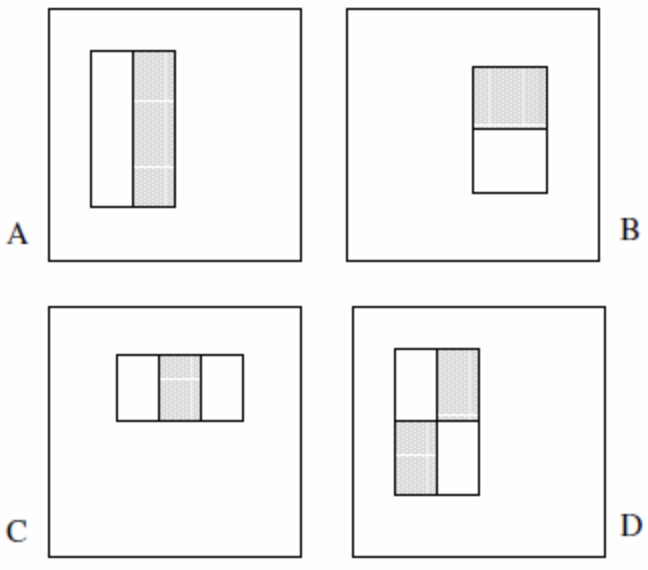
\includegraphics[width = 0.75\textwidth]{./Images/viola-jones.jpg} 
\caption{A set of Haar features used to detect faces in the Viola-Jones method. The pixels in the white regions are summed and subtracted with the pixels in the black region. The algorithm will later decide if a specific feature has been found or not, depending on obtained value.}
\end{center}
\end{figure}

This method is based on the fact that every face shares some basic similarities. Even objects of the same type can share some similarities.\cite{violaJones}
\\\\
Another way to find objects in an image is to try to classify each pixel as either background or foreground, usually referred to as Foreground/Background-segmentation. This usually requires some background knowledge of how the background usually looks like, for example, if the background is grass or a concrete floor.

One of the most basic functions for separating background and foreground is the flood fill method.
Anyone that has used Paint for Windows knows exactly what this one is. It fills a segment of similar pixels with the same color. This method works best on one backgrounds with only one color.
Online there are many different variations but they all accomplish the same goal.\cite{floodFill}
\\\\
Mathematical morphology

Edge detection

Histogram equalisation
\\\\
One possible way of detecting objects in an image is to use depth data, or RGB-D which is depth data embedded in an RGB photo.
A popular device that uses depth data for object detection is the Kinect camera
for Xbox.

On the iPhone X, depth data can be captured by either True Depth on the front camera or with the dual cameras on the back. The True Depth camera works by having a dot projector emit light dots (mainly on a face which is why this feature is found on the front camera) and picking those dots up with an infrared camera.

The dual camera on the back works by taking two photos and comparing those to find the pixel shifts of the same objects. The distance is calculated by \[ \frac{pixelShift} { pixelFocalLength \cdot baselineInMeters}\] and gives the unit in $1/meter$. It is the same principal to how we humans see distance by having two eyes pointing the same direction. \cite{depthMap}

However, obtaining the depth data from the dual cameras in real time is not possible since it requires too much computational power. This unfortunately makes it impossible to use in an ARScene and thus not possible for this project.\\

Despite all the available methods above, object detection without machine learning is still very tricky. These methods work best when the images are in an controlled environment, typically industrial, like finding screws on a white background (as they do in an article posted by combine.se). \cite{combine}
When the environment is a more casual place though, e.g., recognizing furniture indoors, the task becomes much more difficult. For this reason, object detection with pure algorithms is not very common in household applications. Instead object detection with machine learning methods such as R-CNN's (Regional-Convolutional Neural Network) are much more common nowadays.

\section{MATLAB prototype for Object Detection}
\label{sec:ODmatlab}
% Write about design decisions for the Matlab prototype and what it does. 
% Probably add some code as well.
A purely feature based object segmentation method was implemented as a prototype in Matlab. This was done to see if a machine learning model for detecting objects could be dismissed. 
The idea was that if one sent an image into the system, the resulting output would be bounding box coordinates for each respective object within the image. These smaller sub-images would later be separately classified using a deep neural networks. The bounding boxes would also be useful for user interface in the application. 

First, an edge detection method was run on the entire image, to find the edges, which would serve as a good variable for the segmentation. Then, Bradley's threshold algorithm \cite{Bradley} would binarize the image. Bradley's method is locally adaptive and computes the threshold value for each pixel by looking at the mean intensity of a neighborhood of pixels surrounding it.  From this, one can find enclosed blobs, and by finding enclosed blobs containing more than a certain amount of pixels, to remove noisy errors, one can find the objects. The bounding boxes are then found by selecting the minimal and maximal height and weight values of the blobs. See figure \ref{fig:matlabImages} for graphical representation.

\begin{figure}[hbtp]
\begin{center}
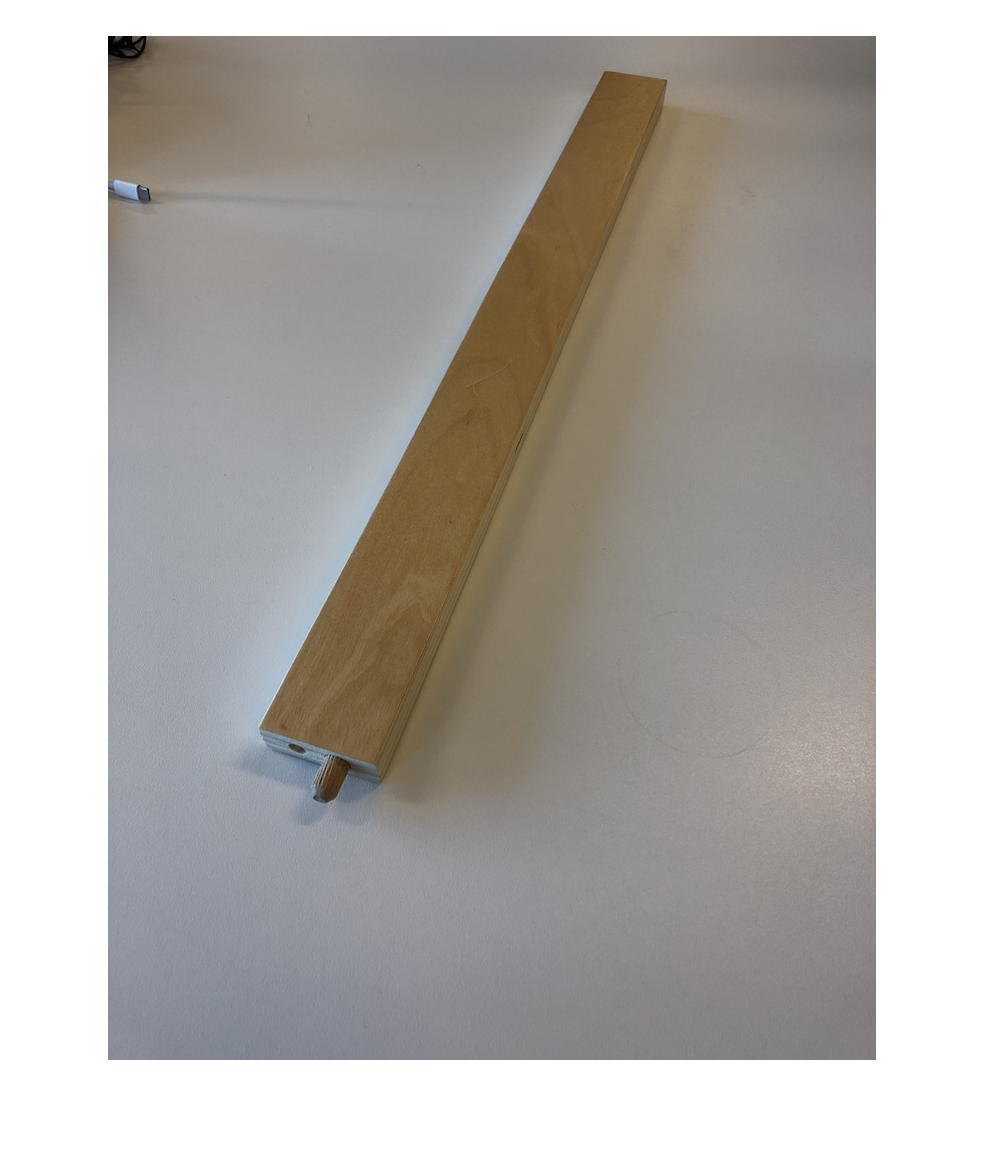
\includegraphics[width = 0.4\textwidth]{./Images/matlabImage1.png}
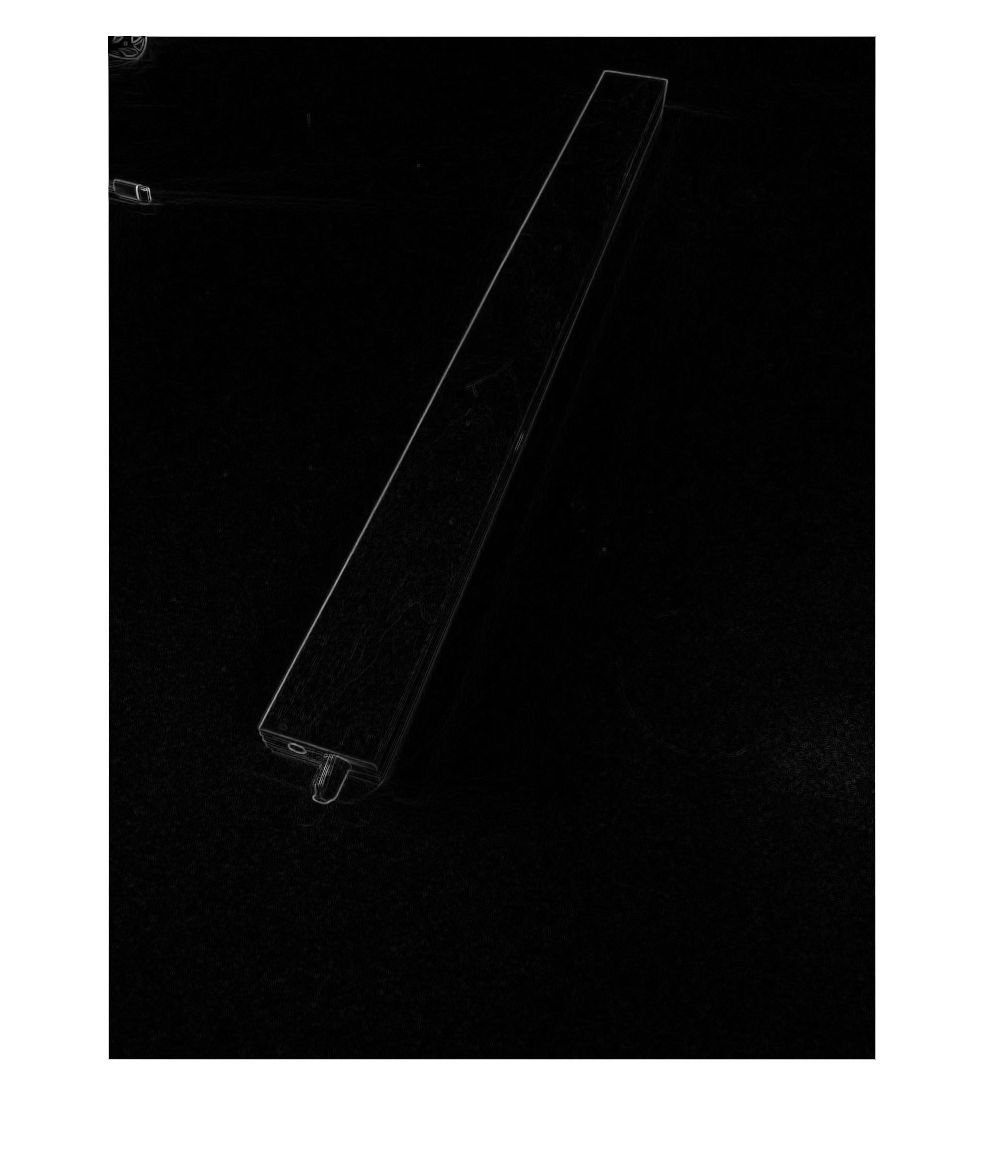
\includegraphics[width = 0.4\textwidth]{./Images/matlabImage2.png}
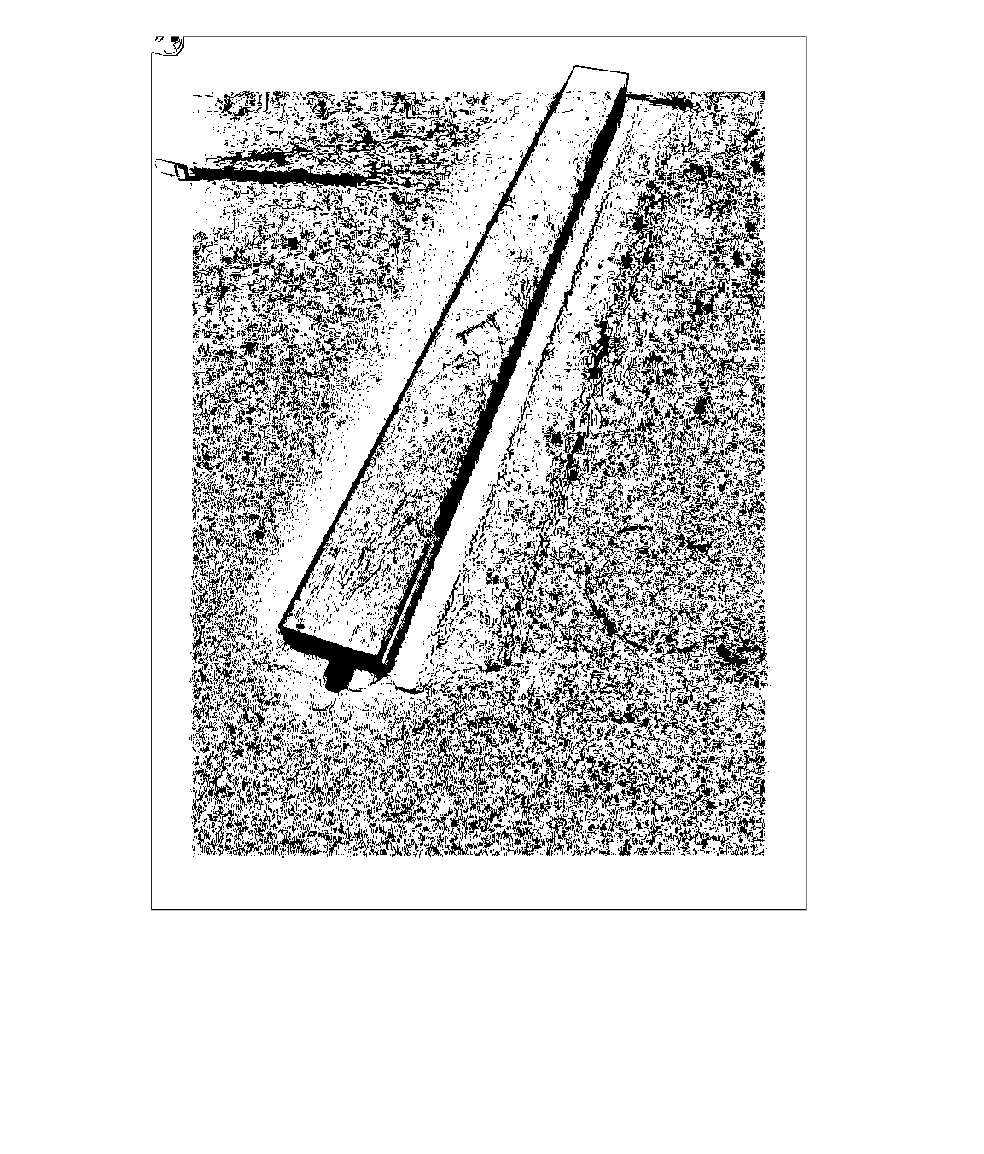
\includegraphics[width = 0.4\textwidth]{./Images/matlabImage3.png} 
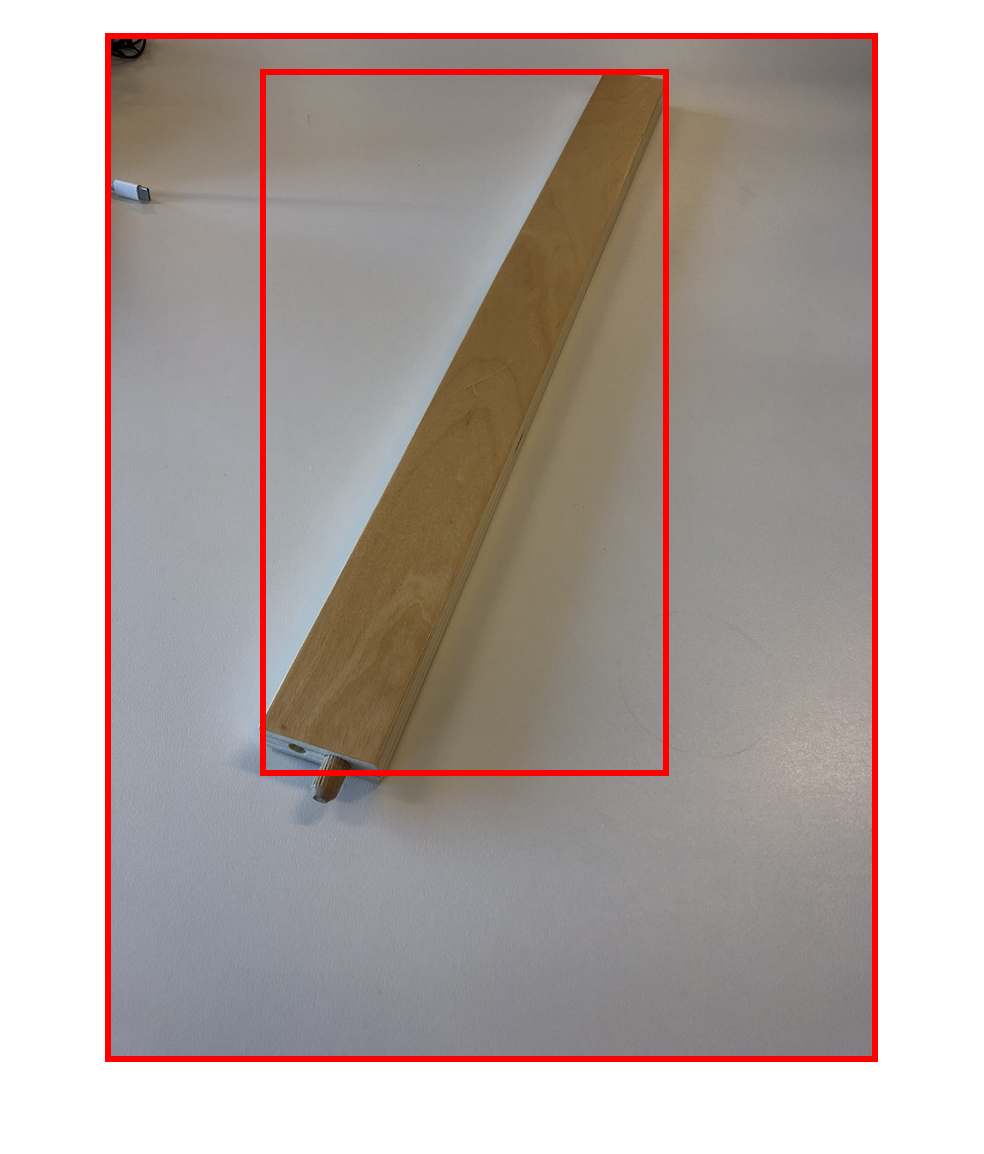
\includegraphics[width = 0.4\textwidth]{./Images/matlabImage4.png} 
\caption{Images showing the results from doing object detection in matlab. Top left image shows the original image. The top right image shows the result from running edge detection on the original image. Bottom left image shows the the result after  binarizing the top right image. the bottom right image shows the generated bounding box superimposed on the original image}
\label{fig:matlabImages}
\end{center}
\end{figure}
[IMAGE FROM WHEN IT DID NOT WORK AS WELL]
This method did however not end up being useful since its performance varied drastically depending on the input image and variables needed to be modified to fit every image. Thus, this method of segmenting out object areas was deemed not viable for this project.

\section{Results from doing object detection in matlab}
\label{sec:ODresults}
A Matlab script was tried in order to find possible ways of segmenting out regions containing objects in an image. The output segments would then each be classified separately. This way we would have both object locations and classifications on each object. \ref{fig:matlabImages} shows an example of this. However, results from this were highly unpredictable and the parameters were too dependent on lighting, shadows, the background among other features. Hence, this method was scrapped.


\newpage
\chapter{One Stage Detector}
After getting stuck for trying to develop a solution that would first do object detection, and then afterward classify the segmented areas separately, it was decided to try a different approach. The one stage detector  \textit{You Only Look Once} method was tried to great success. This chapter will describe how it works, sections \ref{sec:yolo} \ref{sec:mAP}, how the models were created and trained, section \ref{sec:turi}, and then an evaluation of the resulting models in section \ref{sec:turiResults}.

There are other methods of doing object detection and classification, such as \textit{Mask R-CNN} and \textit{Faster R-CNN}, however, they are outside of the scope of this project.
\section{YOLO}
\label{sec:yolo}
YOLO, or You Only Look Once, is a one stage detector approach to object detection and
 recognition \cite{YOLO1}. It takes an image and predicts both bounding boxes and the probabilities of the classes being within these bounding boxes in one run, hence its name. It was designed to be fast and usable in real-time scenarios. Since YOLO sees the entire image during training and testing, it receives contextual information about the classes and reduces error with matching background patches for objects. 
 
 The architecture for \textit{YOLO} consist mainly as a convolutional neural network, with 24 convolutional layers and two fully connected layers. There was also a smaller neural network trained called \textit{Fast YOLO} trained which were only 9 layers which was designed to create an even faster system for object detection. 
 
 The system first divides the input image into an  $S \times S$  grid, where each cell predicts $B$ amount of bounding boxes respectively confidence scores for the boxes. Each bounding box prediction consists of 5 separate predictions: the \textit{x, y} coordinates, represented as their position relative to the the grid cell, width and height relative to the entire image and a confidence value. The confidence values are there to reflect how certain the model is that there exists an object within the box, i.e. ideally, confidence should be zero when no object, and the intersection over union between ground truth and the predicted box if there is. Each grid cell also predicts $C$ probabilities for each class, conditioned that there's an object within the boxes. 
 
 Intersection over union, also known as the Jaccard index, is a way of measuring similarity between sets. It can be written as 
 \[
IOU(A,B) =  \frac{|A\cap B |}{|A\cup B|} =\frac{|A\cap B|}{|A| + |B| - |A \cap B|}
, \quad 0\leq IOU(A,B) \leq 1
 \]
 if $A,B$ are two finite sets. If the two sets are equal, then \[ IOU(A,A) =  \frac{|A\cap A |}{|A\cup A|} = \frac{|A\cap A|}{|A| + |A| - |A \cap A|}  = \frac{|A|}{|A|} = 1 \]
 
 When testing, these scores are then combined to give the class specific confidence values for each of the boxes, thus it receives both the confidence of the class being in the box, and how well the box fits the object. Figure \ref{fig:YOLO_stages} summarizes the flow in YOLO. 
\begin{figure}[hbtp]
\begin{center}
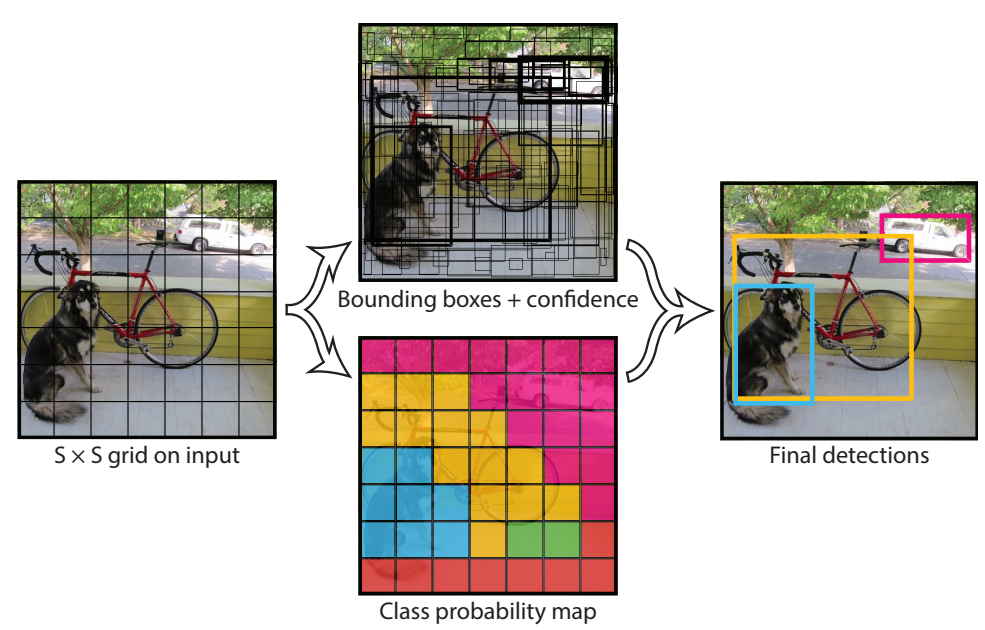
\includegraphics[width = 0.75\textwidth]{./Images/YOLO_stages.PNG} 
\caption{The stages of YOLO. First dives into $S \times S$ grid. Separately predicts bounding boxes with respective confidence, as well as class probability. Then, combines the two to form the final predictions. Image taken from \cite{YOLO1}.}
\label{fig:YOLO_stages}
\end{center}
\end{figure}

Comparisons done by the team working on \textit{YOLO} found that, compared to other real-time systems at the time, both \textit{Fast YOLO} and \textit{YOLO} outperformed them all with \textit{Fast YOLO} being the fastest, but \textit{YOLO} being more accurate on the \textit{PASCAL VOC} data sets \cite{PASCAL}.

Throughout the years Redmon et al. has been working on updating the design pattern of the 
YOLO network. First in 2016 when they introduced \textit{YOLOv2} and then April 2018 with \textit{YOLOv3} \cite{YOLO2}\cite{YOLO3}. \textit{YOLOv2} added a few concepts to the system to make it even more fast and accurate than the earlier iteration. It removed the fully connected layers and it was now possible to train on several different input image resolutions and it could now also predict many more bounding boxes than its predecessor. \textit{YOLOv3} added some changes which improved its ability to detect small objects, with the trade off of having a bit worse performance when finding larger sized objects.  

\section{Mean Average Precision}
\label{sec:mAP}
There is quite a difference when it comes to evaluating a model that does object detection,  compared to normal image classification. When doing the latter, accuracy tells you how often the model makes the correct prediction. However, with object detection it is done differently. The common metric is \textit{mean Average Precision} (mAP).  This metric makes use of the previously discussed \textit{IoU} (Intersection over Union). The IoU and the classification determines if the prediction is deemed correct. The classification obviously has to be the same as the ground truth, and the IoU has to be over a set threshold, these are known as true positives. A predicted box that does not pass the threshold is known as a false positive. If there are more than one prediction that passes the threshold, only one will get seen as a true positive, and the other as false positive. When a prediction was not made for a ground truth box, it is called a false negative \cite{turiAdvanced}.

From the false positives, true positives, and the false negatives, one can calculate recall as well as precision scores \cite{rafaelpadilla}.  Precision is how good the model is to identify only the relevant data, and can be written as
\[ \texttt{precision} = \frac{\texttt{True Positives}}{\texttt{True Positives + False positives }}\]
Recall is how good the model is to find all the relevant data, and is written as 
\[ \texttt{recall} = \frac{\texttt{True Positives}}{\texttt{True Positives +False Negatives }}\]

 When a classification is made you also get a confidence value. One only calls it a prediction if the predictions confidence passes a set threshold. However, if one calculates the recall and precision for all possible thresholds, a Recall x Precision curve can be made. From this curve, one gets the mAP by taking the area under the curve.

There are different standards when calculating the mAP. The PASCAL VOC Challenge uses a mean average precision with a static threshold of 50\%
 \cite{PASCAL}. This is commonly called \textit{mean\_average\_precision\_50}. Another common standard is the one used by COCO  \cite{COCO}. This one calculates the mAP at IoU threshold from 50\%  to 95\%, with increments of 5\% every iteration, and averages them all together. This is quite strangely known as just \textit{mean\_average\_precision}. The latter mentioned method is the one this report will use for evaluation, since it puts more value on localization than the PASCAL VOC method.

\section{Turi Create}
\label{sec:turi}
%Write about the testing an implementation of Turi
Apple has a licenced toolkit for development of custom machine learning models called Turi Create \cite{turiCreate}. This was created to help developers easily implement their own ideas into an app. It includes a methods object detection.

In this project, the object detection method included in Turi Create was tested. First, one
 has to create ground truth data for every image that was trained and tested on. This was
 done using Simple Image Annotator \cite{simpleImage}, where one has to draw bounding
  boxes for the objects in the images and label them; the data output is in the \textit{.csv} format.  Turi Create uses a different format for annotations called \textit{.sframe},
  however, they provide a simple Python script which automatically does the conversion. 

Turi then trains a model using a re-implementation of the TinyYOLO network. It also utilizes transfer learning by starting with an image classifier that has been trained on the imageNet dataset and then does \textit{end-to-end finetuning} to change the network to a \textit{one-stage detector}.

Several models were trained, with different amount of training data, to evaluate how many
 were needed to get a decent result. The Turi website states that at least 30 samples of
each class is needed to generate a good enough model. Hence, we tested for even lower
samples, as well as much more. Lowest amount of training images were around 50, and
highest  were around 1000. The \textit{mean average precision} was measured for each model using 200 testing images, and then plotted to create a graph showing how it
 changed, depending on the amount of training data was used. The results can be seen in section \ref{sec:turiResults}. The best performing model was then to be used in the application.

The code in appendix D.1. shows how the model was created using Turi in python.

The results could also be further inspected by drawing the newly predicted bounding boxes on top of the original image, from this one can visualize how the model actually performed. This was done using code in appendix D.2. Some of the resulting images from different models can be seen in section \ref{sec:turiResults}. 


\subsection{Importing model to application}
After training and evaluating that the model lives up to a standard worth including in this
 project, it was converted to the \textit{.mlmodel} format used in Swift. When inputting a frame from the
application into the model, the model outputs a multi array containing an array for each
  \textit{object} found. These predictions have not been \textit{non-max suppressed}, since that functionality is lost during the conversion from the model used in python, to the .mlmodel format. Thus, it has to be reimplemented in the application itself. 
  A non-max supression threshold of $0.5$ was used as it is considered a traditional standard \cite{nms}. The code in appendix D.3. shows how non-max suppression was implemented. 


\section{Results from doing object detection with Turi}
\label{sec:turiResults}
Because of the vast amount of possible use cases it was decided to scale the objective down. The model was trained only on a few floor backgrounds. 

The mean average precision from the different models that were trained were observed and can be read in table \ref{table:mAP}. These values were plotted, resulting in the graph shown in figure \ref{fig:mAPResult}


\begin{table}[h]
\centering
\begin{tabular}{ |c|c|c| } 
 \hline
 Amount of training images & Percentage of total amount & mean\_average\_precision  \\ 
 \hline
 $\approx 50$& 5\% & 0.17064 \\
 \hline
 $\approx 100$& 10\% & 0.30188 \\
\hline
  $\approx 140$& 15\% &  0.30342 \\
 \hline
 $\approx 185$& 20\% & 0.39269 \\
 \hline
$\approx 280$ &  30\% & 0.41588 \\
 \hline
 $\approx 370$& 40\% & 0.40595 \\
 \hline
 $\approx 415$& 45\% & 0.49917 \\
 \hline
 $\approx 450$& 50\% & 0.47397 \\
\hline
$\approx 570$ & 60\% & 0.50454 \\
\hline
 $\approx 700$& 75\% & 0.54433 \\
 \hline
$926$ & 100\% & 0.57618 \\
 \hline
\end{tabular}
\caption{Mean average precision depending on the amount of training data used.}
\label{table:mAP}
\end{table}

\begin{figure}[h]
\begin{center}
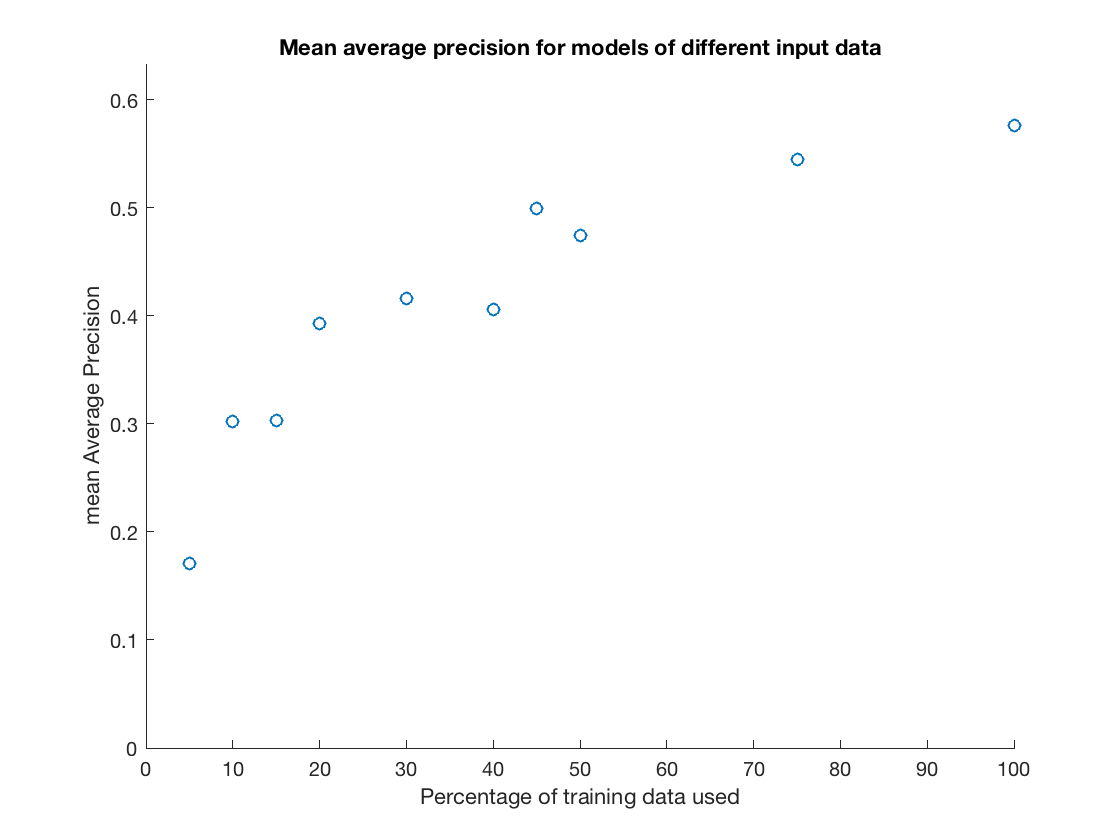
\includegraphics[width = 0.9\textwidth]{./Images/mapPlot.png}
\caption{Mean Average Precision from table \ref{table:mAP} plotted against the amount of training data used. 100\% corresponds to 926 images.}
\label{fig:mAPResult}
\end{center}
\end{figure}

\begin{figure}[h]
\begin{center}
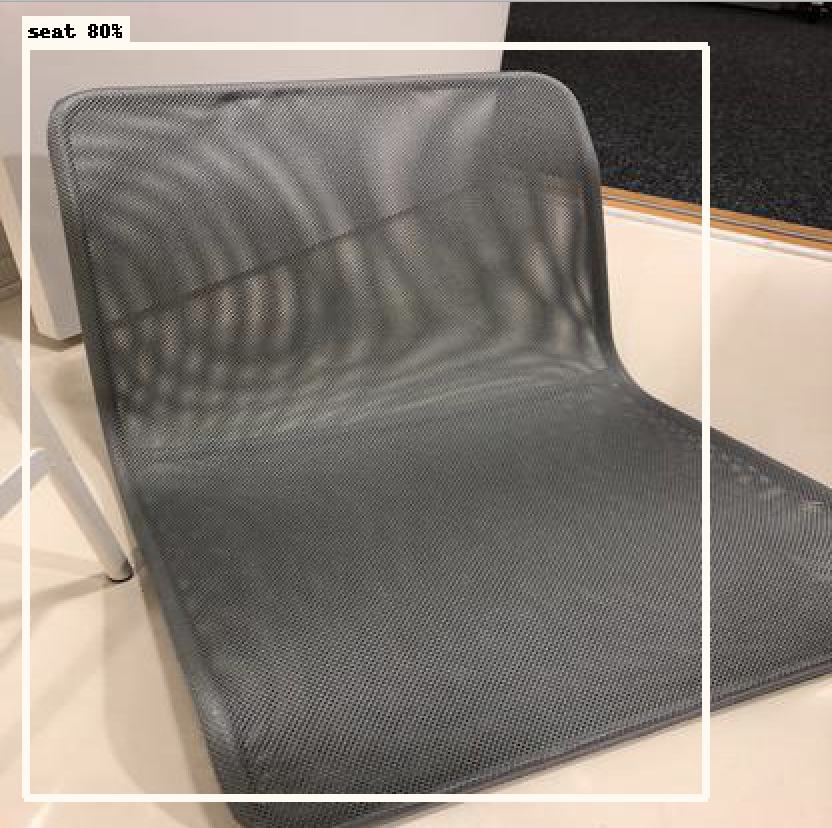
\includegraphics[width = 0.3\textwidth, height = 0.3\textwidth]{./Images/turi100-1.png}
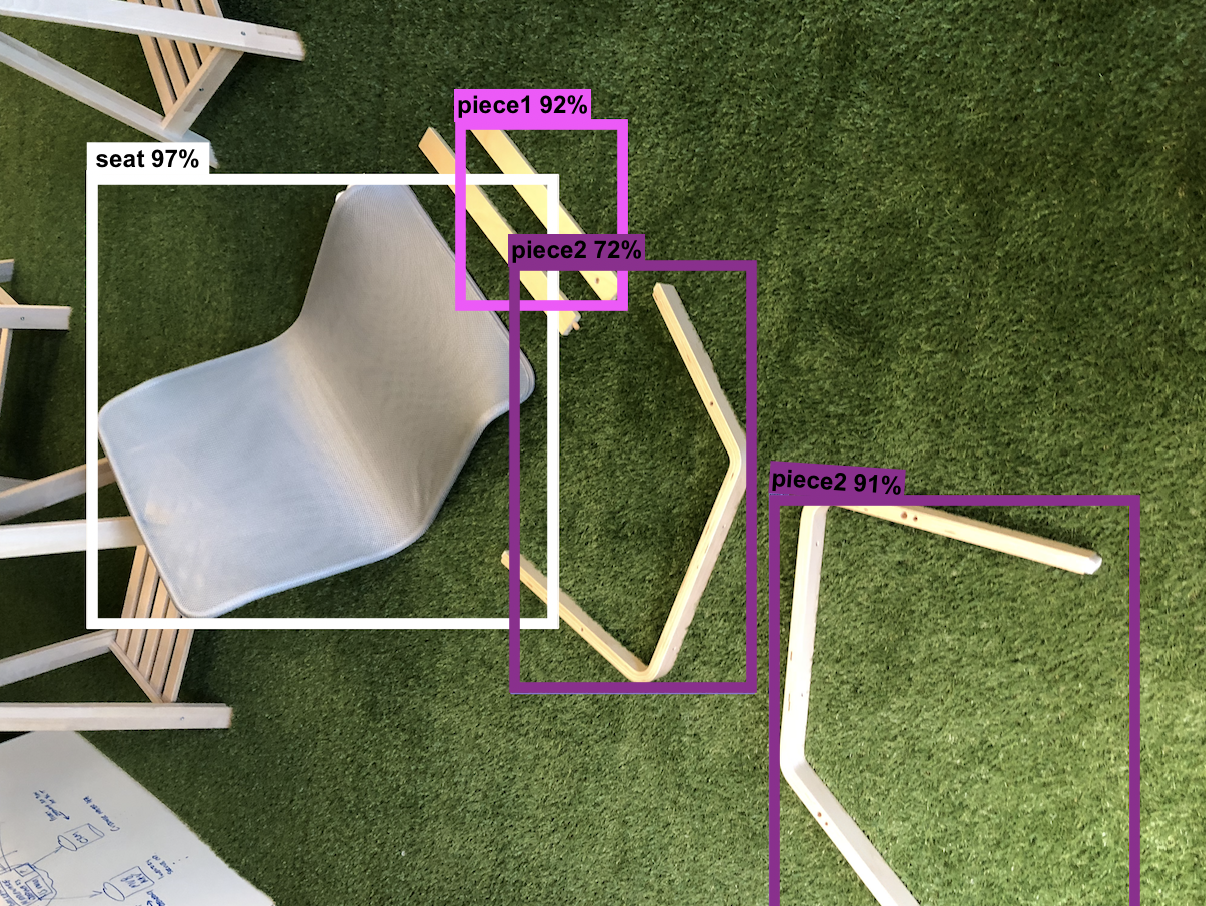
\includegraphics[width = 0.3\textwidth, height = 0.3\textwidth]{./Images/turi100-2.png}
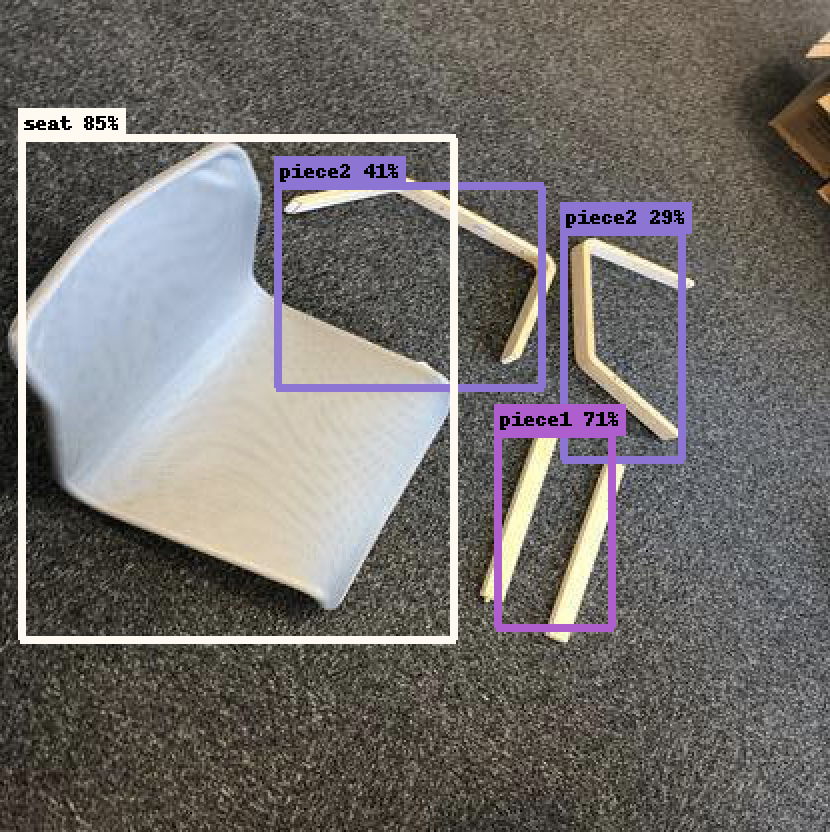
\includegraphics[width = 0.3\textwidth, height = 0.3\textwidth]{./Images/turi100-3.png}
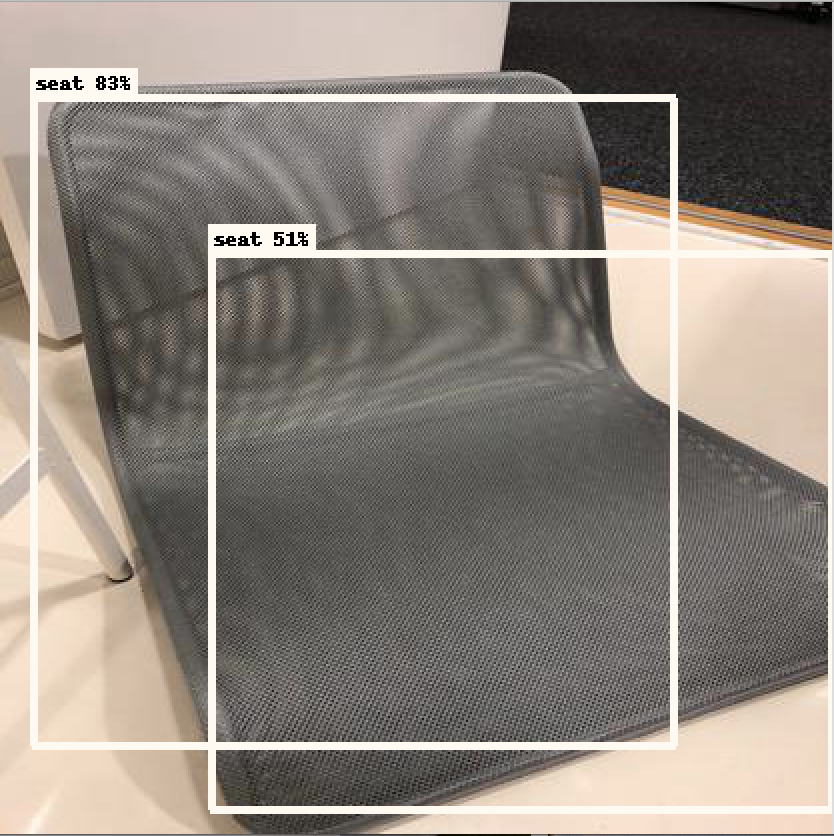
\includegraphics[width = 0.3\textwidth, height = 0.3\textwidth]{./Images/turi015-1.png}
\includegraphics[width = 0.3\textwidth, height = 0.3\textwidth]{./Images/turi015-2.png}
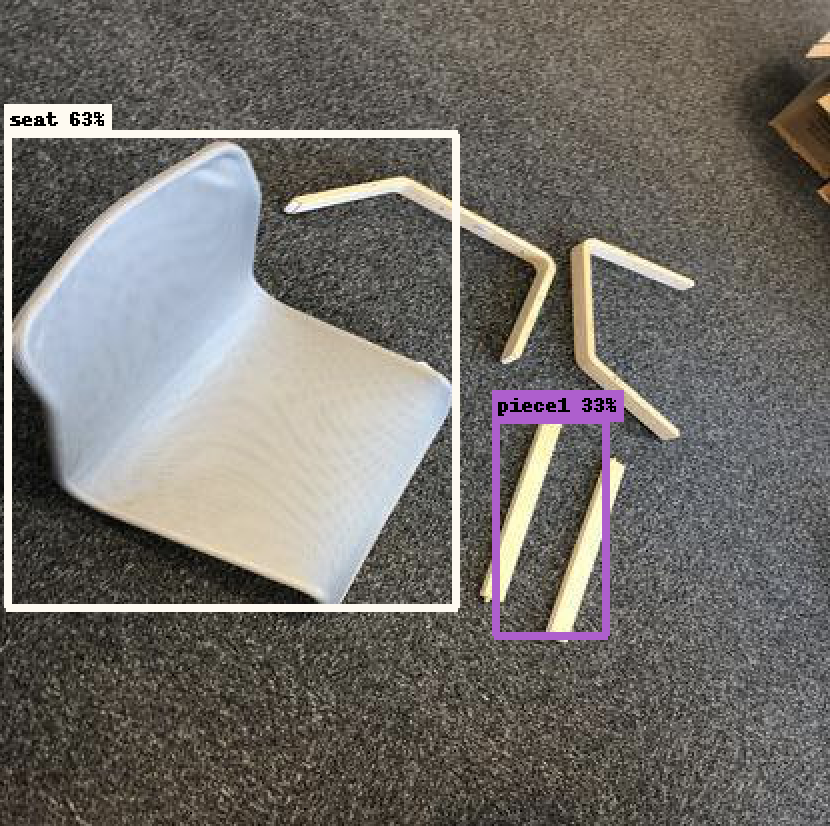
\includegraphics[width = 0.3\textwidth, height = 0.3\textwidth]{./Images/turi015-3.png}
\caption{Images showing how the same three images were classified differently using different models. The top row is classified using the model that was trained on all of the training set. The bottom row shows the images that were trained on only $ 15 \% $ of the training set. }
\label{fig:mAPExamples}
\end{center}
\end{figure}


When training on different amount of data it can appear as if more data gives a worse
result sometimes. That can be explained in two ways. The first explanation is that when
training the models the data was randomly split from the full training data set. That 
means that sometimes there can be more "good" data and sometimes less in the set.
Some images have lots of objects in them and others have fewer. Thus, if you have a
data set with images with lots of objects in them it will likely give better results.
An important thing to mention however is that for the model to perform well it also needs
areas in the image of no object.

The other explanation is that when training, the most optimal model for that data set is
not always, if ever, returned. Take into account early stopping for example.
Sometimes the early stopping can happen on a good place and sometimes it could have
given a better result if the training session would have kept going for a little bit. We did not have a way to use an evaluation set during training, and as such, could not receive training and validation curves. Hence, we can not know how if we trained for too long or too little.

The curve from the tests, fig. \ref{fig:mAPResult}, shows no sign of saturation yet, thus even more data would
surely improve the performance. The reason for not testing with more data is because
of the difficulty of gathering more data (taking photos in different environments and 
adding ground truth data) and the time it took for training.
As of now, the time for training with 926 images on a MacBook Pro 15 inch 2017 with a 2,8 GHz
Intel Core i7 processor is over 24 hours. With half the amount it takes about 17 hours. We would have trained with a GPU, however, it was at the time of training not supported on our hardware.\\

From the graph there is a small plateau between 185 to 370 images. Around that
performance (0.4 mAP) is a sort of minimum for the model to perform well.
For our 6 classes that would correlate to needing around 30-60 images per class.

From the plot in figure \ref{fig:mAPResult} one can see a sharp ascension up until around  20\% of the training set, or 185 images, were used to train the model. This corresponds to roughly 30 images per class. Afterwards, it starts to even out. Hence, the claim that at least 30 images are need to train a somewhat decent model is correct. However, as seen, more data usually generates even better result.

\newpage
\section{Object Tracking}


\subsection{Testing Object Tracking with Vision package}
Vision is a package from Apple which contains a lot of different methods for images and video. It contains still image analysis, image sequence analysis, object tracking, face detection etc.

On their website, Apple has a project that lets any user try out the object tracking on a video. When trying this on one of the furnitures we are going to assemble, the result was very promising. While the parts were laying on the floor and simultaneously moving the camera around, the objects were tracked fairly well. It was only when the camera was moved in such a way that made the pieces rotate in the picture that it started having a hard time tracking it.

For solving this, object detection can be performed in a reasonable time interval and be tracked until object detection is performed once again etc.

\cite{ObjectTracking}
The difference for this project and Apple's test project is that object tracking is going to be performed in real-time. This puts a limit on how many frames per second we can perform object tracking, since in a video playback you can just choose how fast you want to feed the new images. In real-time, the world doesn't stop moving.

After the system was implemented into our application different frame rates were tested. The optimal value was somewhere in-between 10-30 fps. If you went higher than that the application would become very choppy and eventually shut down.

Going lower than 10 fps the user will start to experience that the objects are hard to track in rapid movements.

For this application, however, the user is not going to encounter any scenarios where objects are flying around rapidly. Therefore we will settle for 20 fps as the optimal value for performance since any higher amounts don't really contribute to a better experience.

The following lines of code show how the object tracking was set up. One important thing to realize when setting this up is that the heavy calculations are run on a different thread than the main thread (in this case the work thread). 

That is why they can be executed in a while true loop. Later though, when drawing on the GUI wants to be made, they MUST be done on the main thread.

\begin{lstlisting}[language=swift]
func track()
    {
        cancelTracking = false
        
        var trackingObservations = [UUID: VNDetectedObjectObservation]()
        var trackedObjects = [UUID: ObjectRectangle]()
        let requestHandler = VNSequenceRequestHandler()
        let boundingFrame = delegate?.getBoundingFrame()
        for object in objectsToTrack
        {
            let observation = VNDetectedObjectObservation(boundingBox: object.getNormalizedRect(frame: viewFrame))
            trackingObservations[observation.uuid] = observation
            trackedObjects[observation.uuid] = object
        }
        
        while true
        {
            if cancelTracking { break }
            
            var rects = [ObjectRectangle]()
            var trackingRequests = [VNRequest]()
            
            guard let frame = delegate?.getFrame() else {
                usleep(useconds_t(millisecondsPerFrame * 1000))
                continue
            }
            
            for trackingObservation in trackingObservations
            {
                // Create the requests
                let request = VNTrackObjectRequest(detectedObjectObservation: trackingObservation.value)
                request.trackingLevel = .fast
                trackingRequests.append(request)
            }

            try? requestHandler.perform(trackingRequests, on: frame, orientation: CGImagePropertyOrientation.up)

            for processedRequest in trackingRequests
            {
                // Handle the results from the requests
                guard let observation = processedRequest.results?.first as? VNDetectedObjectObservation else { continue }
                
                if observation.confidence > confidenceThreshold
                {
                    guard let object = trackedObjects[observation.uuid] else { continue }
                   // Set new bounding box
                    object.setNewBoundingBox(newBoundingBox: observation.boundingBox, frame: boundingFrame)
                    trackedObjects[observation.uuid] = object
                    trackingObservations[observation.uuid] = observation
                    
                    rects.append(object)
                }
            }

            DispatchQueue.main.async {
                rects = rects.sorted { $0.name! < $1.name! }
                self.delegate?.trackedRects(rects: rects)
            }
            
            // The tracking will stop if no observation has a high confidence value
            if rects.isEmpty
            {
                DispatchQueue.main.async {
                    self.requestCancelTracking()
                    self.delegate?.trackingLost()
                }
            }

            usleep(useconds_t(millisecondsPerFrame * 1000))
        }
        
        DispatchQueue.main.async {
            self.delegate?.trackingDidStop()
        }
    }
\end{lstlisting}


\subsection{Combining Object detection with Object Tracking}
The purpose of having the object tracker is to be able to avoid performing object detection and object recognition 30 frames per second or so. Also, doing this with R-CNN and Yolo nets have shown choppy results where an object can be identified in one frame, not identified in the next and then again identified.
There is no real issue with this since both solutions perform really well overall. There is however concerns for the end user to have a fluid experience.

One way to solve this is to perform the detection and recognition once, to later continue to track the position of those items with a cheaper algorithm.
Object detection and recognition will then be repeated, but only update the state of the rectangles if the correct objects are identified.
In this application, an arrow was drawn between the objects with an instructional text for the user. Doing this created a rather big issue though.

\begin{figure}[!hbtp]
\begin{center}
\includegraphics[width = 0.35\textwidth]{./Images/tracking.png}
\caption{The image shows an early stage of the application were two pieces have been recognized by the network and an outline around them has been drawn. Between them, an arrow is rendered on the floor, showing how to put together the two pieces. The objects are continuously being tracked within the frame and the arrow is also updated.}
\label{fig:tracking}
\end{center}
\end{figure}

In this project, ARKit by Apple has been utilized. As previously stated, when working with ARKit, a frame from the camera is fetched by either calling snapshot() on the ARSCNView object or getting the currentFrame from the ARSession.
However, both of these images contain both the RAW camera image and all the virtual items rendered in the ARScene. We did not find a way to capture just the RAW camera image.

This whole scenario created a kind of positive feedback loop because the virtual arrow that was rendered between the objects was usually contained within either one of the tracking rectangles. Thus, the arrow's position was determined by the tracking rectangle and the tracking rectangle was tracking the position of the arrow.
Just the tiniest change in the picture made the arrow jump up and down until it finally got out of frame.

The take away from this was to skip object tracking and solve the problem in another way.

An assumption was made that just as talked about before, the furniture parts are laying still on the ground while the user is using the application. That means that we can rely on ARKit to keep track of where the object is for us instead.

Switching gear to that solution made the whole application much better and easier to code. A takeaway from that is that adding more technology to a project does not always equal a better product. Sometimes it is better to use the components the way they are meant to be used and try not to make it more complicated than it needs to be.

CAN ELABORATE MORE ON THIS IN THE CONCLUSIONS

\newpage
\chapter{The Finished Application}
This chapter will round off the work process of the report. It goes through how the final application was designed and implemented in \ref{sec:Application}. The chapter then ends with section \ref{sec:usertest}, detailing the evaluation process of the application, which was the by having users test the finished application.

\section{The iOS Application}
\label{sec:Application}
The application is build for iOS using Xcode and Swift 4.0. The app has been developed specifically for iPhone X. It has also only been tested on iPhone X. However, the app should work on other iPhone models that support ARKit 2.0 as well.

\subsection{Class diagrams}
Below are some class diagrams for the reader to better understand what different parts there are, 
how they fit together and how the application works as a whole. The diagrams are divided into 
three parts to be readable in the paper.

\begin{figure}[!hbtp]
\begin{center}
\includegraphics[width = 1.1\textwidth]{./Images/AssemblerClassDiagram1.jpg}
\caption{A class diagram of the assembler view part of the application. The Furniture class in the lower right is incomplete and is shown in the next diagram.}
\label{fig:classdiagramassembler}
\end{center}
\end{figure}

The application follows the Model View Controller design pattern as well as the Delegate design pattern.
This decision was made since many tools and features in iOS and Swift are implemented that way,
so we are just following the standard procedure.

\textbf{AssemblerViewController} is the controller for the view that holds the ARSCNView.
It is responsible for what happens when the user taps on a button in that view and displaying the correct
information to the user at the right times. It also holds the \textbf{Instruction Executioner} which holds a 
set of instructions that it gets at initialisation. The instruction executioner executes the current
instruction and therefore decides what will happen when it executes. Every instruction is executed on a worker queue thread to avoid the video feedback to freeze during execution.\\

The InstructionExecutioner holds the \textbf{ObjectDetector} which finds specific objects in a 
trained model from a pixel buffer. The found objects are passed back as \textbf{ObjectRectangles} through the delegate. The object rectangles are bounding boxes
of the objects on screen. They are represented as CGRect's and can be stored and fetched as
either regular or normalized rectangles. The normalized variants are needed in all kinds of machine learning purposes and the regular form are used in all GUI purposes, such as in the \textbf{OverlayView}. (Normalized 
rectangles have values of 0-1 for widths, heights, x-, and y-position. The origin is in the lower left 
corner.)\\

The \textbf{AssemblerModel} is the model in the AssemblerViewController, but is also used in the InstructionExecutioner since they are highly dependent on each other.
The most important attributes it holds are the \textbf{ObjectParts} that have been spotted by the 
app during the execution of the current instruction.
That way, all the parts needed for the current instruction do not need to be in the same image 
together but instead can be spotted separately.\\

\begin{figure}[!hbtp]
\begin{center}
\includegraphics[width = 0.9\textwidth]{./Images/FurnitureClassDiagram.jpg}
\caption{A class diagram of the furniture selection views part of the application. The Furniture class.}
\label{fig:classdiagramfurniture}
\end{center}
\end{figure}

The furniture that the user wants to put together is selected in a collection view \textbf{FurnitureSelectionViewController}
which conforms to the UICollectionViewDelegate- and UICollectionViewDataSource protocol for the collection view functionality.
The data to be viewed in the controller is fetched from the \textbf{Database} class.
The return data from the class are hardcoded from the start but can easily be changed to fetch
data from a server.\\

The \textbf{Furniture} holds all the information about a specific furniture as well as the instruction set of how to put it together. The instruction set consists of \textbf{Instruction}'s that can be
of the kind \textbf{ScanInstruction}, \textbf{AssembleInstruction} or \textbf{CompleteInstruction}.
A regular Instruction is usually just text instructions to the user, while the scan instructions tell the instruction executioner to look for specific parts during that step.
The assemble instruction is run when the user is in the process of assembling two parts.
Finally the complete instruction is given which tells the executioner that the furniture has been fully assembled.\\

For scanning barcodes, the \textbf{BarcodeScannerViewController} is used, which inherits all the photo capture functionality from the \textbf{ImageViewController}.\\

\begin{figure}[!hbtp]
\begin{center}
\includegraphics[width = 0.5\textwidth]{./Images/UtilitiesClassDiagram.jpg}
\caption{A class diagram of the utilities part of the application. These are some classes that make the rest of the code in the application easier to understand and use.}
\label{fig:classdiagramutilities}
\end{center}
\end{figure}

In the utilities folder there are some classes that simplifies the rest of the application
by holding code that removes a lot of redundancy.

The \textbf{GeometryFactory} creates all the 3D geometry for the ARScene and return the nodes 
containing this geometry. An example is that it can create all the furniture parts as virtual object 
nodes to be placed in the scene.

A lot of conversion between pixel buffers and UIImage's are made and the \textbf{ImageConverter }
eases the pain of having to do that in many places.

Finally the \textbf{Prediction} class helps the object detector when getting results
from the VNCoreMLRequest.

\subsection{Connecting two pieces in AR}
After finding the specific pieces that are supposed to be connected they are created as
virtual objects in the scene on their respective locations. The location is determined using
hit tests of the screen positions to the detected plane from the ARScene.

The virtual objects are rendered in the scene using SCNNode's as talked about in \ref{subsecARKit} and the node position is the origin of the 3D model. The origin has been chosen to be at a location that is touching the floor when it is standing. That way they can easily be placed to look like they are standing right on the floor.
When both pieces are placed in the scene they are to be moved with an animation in a way so that they become connected.

Each virtual object node can embed another node called the "anchor point". The position of this node within the parent node is where the other object is to be connected. To connect them, either the object without the anchor point moves to the anchor point position, or the two object move so that each of their anchor points are at the same position.
This is accomplished using the algorithm below.

\begin{lstlisting}[language=swift]
    var furniturePartNodes = [SCNNode]()

        for object in model.foundObjects
        {
            guard object.name != nil else { return }
            guard object.position != nil else { return }
            
            let furnitureNode = addFurniture(part: object.name!, position: object.position!)
            furniturePartNodes.append(furnitureNode)
        }
        
        var previousNode: SCNNode? = nil
        var previousAnchorPoint: SCNNode? = nil
        
        var nodeActions = [(SCNNode, [SCNAction])]() // A list for storing animations to run on a node later
        
        for node in furniturePartNodes
        {
            var actions: [SCNAction] = []
            actions.append(SCNAction.rotate(by: -CGFloat.pi / 2, around: SCNVector3(0, 0, 1), duration: 1))

            let anchorPoint = node.childNode(withName: ANCHOR_POINT, recursively: true)
            
            if anchorPoint == nil
            {
                if previousAnchorPoint != nil
                {
                    actions.append(SCNAction.move(to: previousAnchorPoint!.worldPosition, duration: 2))
                }

                previousNode = node
            }
            else
            {
                previousNode?.runAction(SCNAction.move(to: anchorPoint!.worldPosition, duration: 2))
                if previousAnchorPoint != nil
                {
                    actions.append(SCNAction.move(to: previousAnchorPoint!.worldPosition, duration: 2))
                    actions.append(SCNAction.move(by: node.worldPosition.substract(other: anchorPoint!.worldPosition), duration: 2))
                }

                previousAnchorPoint = anchorPoint
            }
            
            // HACK: Adds an extra action with no content at the end to make completion handler wait until the last action is done
            actions.append(SCNAction.move(by: SCNVector3Zero, duration: 1))
            
            nodeActions.append((node, actions))
        }
}
\end{lstlisting}

Afterwards, the items in 'action' are performed on the respective node.

\subsection{The finished GUI}
The finished GUI is similar to the prototype but some details are different. The resulting screen shots
can be seen in figure \ref{fig:applicationSelection} and \ref{fig:applicationAssembler}.

\begin{figure}[!hbtp]
\begin{center}
\includegraphics[width = 0.3\textwidth]{./Images/Application1}
\includegraphics[width = 0.3\textwidth]{./Images/Application2}
\includegraphics[width = 0.3\textwidth]{./Images/Application3}
\caption{Images from the use of the application when selecting a furniture and right before starting the assembler view.}
\label{fig:applicationSelection}
\end{center}
\end{figure}

\begin{figure}[!hbtp]
\begin{center}
\includegraphics[width = 0.3\textwidth]{./Images/Application4}
\includegraphics[width = 0.3\textwidth]{./Images/Application5}
\includegraphics[width = 0.3\textwidth]{./Images/Application6}
\caption{Images from the application when having started the ARScene, finding objects and showing animations when putting them together. The green rectangle on the floor is an indication that the part has been recognized by the application. We call these markings.}
\label{fig:applicationAssembler}
\end{center}
\end{figure}

\section{User Testing}
\label{sec:usertest}
Evaluating the AR experience is possible on a technical level, to research if the 
combination of AR with object recognition is feasible. This can be done by, for instance,  
making sure the application is running at an acceptable frame rate. However, as this 
report also wants to research into the desirability of this combination of technology, the 
same approach is not as appropriate. What was done was to test the 
application ourselves, as well as get outside evaluations through user tests.

The user tests were set up by having people from the office sign up online to come test our 
application, as well as answering a form afterwards where they answered several 
questions. While the users were doing the tests, they were observed and comments were 
written down, reporting on how they behaved. 

The form asked the participants the following questions:
\begin{itemize}
\item Did you know that you could skip instructions?
\item How easy was it to understand how to get to the next step?
\item How easy was it to understand how the pieces fit together?
\item How easy did you feel the app was to use?
\item Compared to using paper instructions, did the app make it easier to understand how to put together the furniture? ? If not, then why?
\item What potential do you see in this app?
\item General feedback
\item Suggestions of improvement
\item What is your role at Jayway?
\end{itemize}

A user survey was done in order to evaluate the performance of the application. By having a multitude of interested people booking time slots for a ten minute testing period, a decent amount of sample data could be gathered and evaluated. Figures \ref{fig:question1} to \ref{fig:question6} show bar charts and pie charts representing the answers gathered from the participants to some of the questions they were asked. 

\begin{figure}[hbtp]
\begin{center}
\includegraphics[width = 0.9\textwidth]{./Images/easyToGetToNext.png}
\caption{Results from when users were asked "How easy was it to understand how to get to the next step?". X axis is their rating from 1-5 and y axis is how many.}
\label{fig:question1}
\end{center}
\end{figure}

\begin{figure}[hbtp]
\begin{center}
\includegraphics[width = 0.9\textwidth]{./Images/easyToUnderstand.png}
\caption{Results from when users were asked "How easy was it to understand how the pieces fit together?". X axis is their rating from 1-5 and y axis is how many}
\label{fig:question2}
\end{center}
\end{figure}

\begin{figure}[hbtp]
\begin{center}
\includegraphics[width = 0.6\textwidth]{./Images/knowToSkip.png}
\caption{Results from when users were asked "Did you know that you could skip instructions?"}
\label{fig:question3}
\end{center}
\end{figure}

\begin{figure}[hbtp]
\begin{center}
\includegraphics[width = 0.9\textwidth]{./Images/easyToUse.png}
\caption{Results from when users were asked "How easy was it to understand how to get to the next step? X axis is their rating from 1-5 and y axis is how many"}
\label{fig:question4}
\end{center}
\end{figure}

\begin{figure}[hbtp]
\begin{center}
\includegraphics[width = 0.6\textwidth]{./Images/comparedTo.png}
\caption{Results from when users were asked "Compared to using paper instructions, did the app make it easier to understand how to put together the furniture?"}
\label{fig:question5}
\end{center}
\end{figure}

\begin{figure}[hbtp]
\begin{center}
\includegraphics[width = 0.9\textwidth]{./Images/potential.png}
\caption{Results from when users were asked "What potential do you see in this app? X axis is their rating from 1-5 and y axis is how many"}
\label{fig:question6}
\end{center}
\end{figure}


By collecting the data from the forms, the recorded videos and our own observations we could find some general trends and reach a few conclusions.

What we found was that half of the participants thought it was easier to use our
application to assemble the furniture than using a traditional paper instruction, and no-one
thought it was definitively more difficult, as seen in figure \ref{fig:question5}. This could be due to the fact that the piece of furniture we 
chose to train on were quite simple to assemble, relative to other possible furniture. It would be interesting to perform the same task but on a more complicated piece of furniture.

Every participant thought that the application had good or great potential, see figure \ref{fig:question6}, if it were 
to be improved. This result shows that the use of this technology is mostly desirable, if 
done in a more proper way.

The answers show that most people could understand how to use the application and 
could intuitively start up the application and start the assembly process without outside 
help, shown in figure \ref{fig:question1}, \ref{fig:question2} \& \ref{fig:question4}. In some cases we noticed that people were a bit confused with the augmented reality 
interface. Several participants had a hard time understanding the purpose of the green 
rectangles that were rendered around a found object in the scene. Mostly because the 
rectangles were significantly larger than the object itself, hence, it often overlaps with 
other objects on the floor.

The hassle of having to put the phone down in between looking at the animation and 
actually assembling the furniture parts was also brought up. Some of the participants had 
to pick up the phone several times during certain steps to make sure they were executing 
the task in the correct manner.

At times, some participants were getting confused because the application could not find 
the correct parts. This happened because of several reasons. One being that they had 
accidentally skipped an instruction, thus the application were looking for model parts that 
had not yet been assembled. Another reason being that the machine learning model were 
inconsistent at times and could not identify certain in the orientation it was currently in. It 
also happened when the users did not perform 
the first task given by the application, being that they had to make sure that the parts were 
laying on the floor and not overlapping each other. A solution to these problems could be 
to give the users a more clarified and more intuitive set of instructions such that the user 
don't accidentally skip an important instruction. Another solution is to retrain the machine 
learning model to be able to identify the parts in more orientations. 

The user test was performed in the Jayway offices on people with background in 
technology, where most participants were developers or designers. Due to this, the result 
could be skewed, since people with similar background have a tendency to understand 
each others intent. The same test would have to be performed on actual end users with a 
more varied background to see if it would match the results we've gathered.
\newpage
\section{Conclusion}

\subsection{Result from tracking}

How well it tracked objects and how many it could track at the same time.

\subsection{Analysing training different configurations and their charts}

Different model configuration and the test results. Charts of accuracy and loss.

\subsection{Results from doing object detection in matlab}

\subsection{Results from doing object detection with Turi}

\subsection{Results from doing R-CNN}

\subsection{Rendered nodes in ARScene and how stable they were}
Precision when doing the hit tests

How well the nodes stayed in their place (depending on environment?)

\subsection{Overall performance of the app}

What is the peek performance?



\newpage
% As we go on we decide on what we will write here.

\begin{thebibliography}{X}

\bibitem{nms}
Jan Hosang, Rodrigo Benenson, Bernt Schiele \textit{Learning non-maximum suppression}, Max Planck Institut für Informatik, Saarbrücken, Germany (9 May 2017)
\url{https://arxiv.org/pdf/1705.02950.pdf}

\bibitem{facebookAR}
TechCrunch, \textit{Facebook's Head Of Augmented reality on its plans for AR glasses}
Published on Oct 24, 2018
https://youtu.be/JEGqc9wzC0o?t=1041

\bibitem{videoplace}
Myron Krueger - Videoplace, Responsive Environment
\url{https://www.youtube.com/watch?v=dmmxVA5xhuo}

\bibitem{slam}
SLAM: Simultaneous Localization and Mapping - Wolfram Burgard, Cyrill Stachniss, Kai Arras, Maren Bennewitz
\url{http://ais.informatik.uni-freiburg.de/teaching/ss12/robotics/slides/12-slam.pdf}

\bibitem{iphoneslam}
Seene SLAM Technology - culturengine
\url{https://www.youtube.com/watch?v=434SsV9nGHc}

\bibitem{microsoft}
Microsoft HoloLens, Software Asset Management – Microsoft SAM, Microsoft
\url{https://www.microsoft.com/en-us/hololens}

\bibitem{overfitting}
Beware of overfitting and underfitting, O'Reilly
\url{https://www.oreilly.com/library/view/scala-and-spark/9781785280849/3c1c7845-811d-47b9-a54f-c2584fe930b3.xhtml}

\bibitem{violaJones}
Face Detection System Based on Viola - Jones Algorithm, Mehul K Dabhi1, Bhavna K Pancholi2
\url{https://pdfs.semanticscholar.org/f63c/fcdd63bd34bcd6ec028169e6fe144e9cc83c.pdf}

\bibitem{floodFill}
Lode's Computer Graphics Tutorial - Flood Fill, Lode Vandevenne
\url{https://lodev.org/cgtutor/floodfill.html}

\bibitem{depthMap}
AVDepthData, Apple Documentation
\url{https://developer.apple.com/documentation/avfoundation/avdepthdata}

\bibitem{combine}
Object recognition without deep-learning, Combine
\url{http://combine.se/object-recognition-without-deep-learning/}

\bibitem{extremeProgramming}
Extreme Programming
O'Reilly Media
ISBN-13: 978-0596004859

\bibitem{appleAR}
Augmented Reality, Apple
\url{https://www.apple.com/lae/ios/augmented-reality/}

\bibitem{ARScanning}
Scanning and Detecting 3D Objects, Apple
\url{https://developer.apple.com/documentation/arkit/scanning_and_detecting_3d_objects}

\bibitem{ObjectTracking}
Tracking Multiple Objects or Rectangles in Video, Apple
\url{https://developer.apple.com/documentation/vision/tracking_multiple_objects_or_rectangles_in_video}

\bibitem{NIPS2009_3766}
Region-based Segmentation and Object Detection
S. Gould, T. Gao and D. Koller, in \textit{Advances in Neural Information Processing Systems 22}, 
ed. Y. Bengio and D. Schuurmans and J. D. Lafferty 
and C. K. I. Williams and A. Culotta, 
pp 655--663
(2009)
\url{http://papers.nips.cc/paper/3766-region-based-segmentation-and-object-detection.pdf}

\bibitem{MARS}
D. Chatzopoulos, C. Bermejo, Z. Huang and P. Hui, "Mobile Augmented Reality Survey: From Where We Are to Where We Go," in \textit{IEEE Access}, vol. 5, pp. 6917-6950, 2017.
doi: 10.1109/ACCESS.2017.2698164
\url{http://ieeexplore.ieee.org/stamp/stamp.jsp?tp=&arnumber=7912316&isnumber=7859429}

\bibitem{googleGlasses}
Glass Explorer Edition, Google Developers, Google
\url{https://developers.google.com/glass/}

\bibitem{pokemonGO}
Pokémon GO, NIANTIC
\url{https://www.pokemongo.com/en-us/}


\bibitem{IKEAPlace}
IKEA Place, App Store, IKEA Systems B.V, (2017)
\url{https://itunes.apple.com/us/app/ikea-place/id1279244498?mt=8}

\bibitem{fieldbit}
Fieldbit Hero, FieldBit
\url{https://www.fieldbit.net/products/fieldbit-hero/}

\bibitem{deepLearningTutorial}
Yann LeCunn, Marc'Aurelio Ranzato, Deep Learning Tutorial, ICML, Atlanta, (2013), 
\url{https://cs.nyu.edu/~yann/talks/lecun-ranzato-icml2013.pdf}

\bibitem{YOLO1}
Joseph Redmo, Santosh Divvala, Ross Girshick, Ali Farhadi (2016), University of Washington
, Allen Institute for AI
, Facebook AI Research
You Only Look Once: Unified, Real-Time Object Detection
\url{https://arxiv.org/pdf/1506.02640.pdf} 

\bibitem{YOLO2}
Joseph Redmon, Ali Farhadi, \textit{YOLO9000:
Better, Faster, Stronger}, 
University of Washington \& Allen Institute for AI (2016)
\url{https://arxiv.org/pdf/1612.08242.pdf}

\bibitem{YOLO3}
Joseph Redmon, Ali Farhad
\textit{YOLOv3: An Incremental Improvement}
University of Washington (2018)
\url{https://arxiv.org/pdf/1804.02767.pdf}

\bibitem{PASCAL}
The PASCAL Visual Object Classes
\url{http://host.robots.ox.ac.uk/pascal/VOC/}

\bibitem{digi-capital}
Digi-Capital. \textit{Ubiquitous  \$90 billion AR to dominate focused \$15 billion VR by 2022}
(January 26, 2018)
\url{https://www.digi-capital.com/news/2018/01/ubiquitous-90-billion-ar-to-dominate-focused-15-billion-vr-by-2022/}

\bibitem{Bradley}
Derek Bradley, Gerhard Roth, \textit{Adaptive Thresholding Using the Integral Image},
Carleton University, Canada \& National Research Council of Canada (2005), 
\url{http://people.scs.carleton.ca/~roth/iit-publications-iti/docs/gerh-50002.pdf}

\end{thebibliography}



\end{document}